\chapter{Final Design}
\section{Overview}
Now that a wealth of valuable experience has been gathered through simulations and extensive testing,
a specific microphone type has been selected and an optimal array geometry for this project's use case has been identified.
This selection process was critical for achieving the project's goal of designing a fully functional, professional end product.
This chapter outlines the final design of the sound source localization system.

In the research detailed in section \ref{sec:array_prototype_measurements},
a key hypothesis emerged regarding the potential for improved sound source localization with a three-dimensional array structure as compared to a planar geometry.
This led to the development of a new mechanical concept, which is detailed later in this chapter.

For the system to function independently, it was essential to incorporate all necessary components within the design.
However, due to the computational intensity of beamforming algorithms, they cannot be processed on a microcontroller like the Teensy 4.1.
Consequently, the design had to accommodate external processing capabilities.

Another significant consideration was that a single microphone array could only provide a directional vector of located sound sources without information about the distance to these sources.
To pinpoint an object's location accurately, multiple microphone arrays are needed.
This requirement necessitated a design that allows for easy integration with a centralized computer or server, capable of connecting to multiple microphone arrays.

The optimal solution was to design a system that could stream all lossless audio data from each microphone array to the server in real-time.
Such a design ensures maximal flexibility, as it allows to apply basically any sort of localization algorithm on the server side.
In addition, it enables the usage of multiple microphone arrays, which can be placed at different locations, thus increasing the overall accuracy of the system.
\newpage

\subsection{Key Requirements}
The following key requirements have been set:
\begin{itemize}
	\item Simultaneous streaming of 32 microphone channels in real-time
	\item Lossless audio transmission with a sampling rate of 44.1\,kHz and 16\,bit resolution
	\item \acrshort{gnss} \acrshort{rtk} receiver for accurate positioning and timing information
	\item \acrshort{imu} for geographic heading and leveling information
	\item Ambient pressure and temperature sensor for calculating the exact speed of sound
	\item Ethernet interface for audio streaming and device configuration
	\item \acrshort{poe} power supply for single cable operation over long distances (up to 100\,m)
	\item Intuitive \acrfull{gui} for device configuration and monitoring
	\item Flexible mounting option for installation on a standard camera tripod
	\item Microphone integration that is resistant to the influence of wind
	\item Adjustable array arm angle for optimal beamforming performance
	\item \acrshort{rgb} \acrshort{led}s for visual feedback and status indication
\end{itemize}

\subsection{Key Decisions}
The following section describes the key decisions made during the development of the final design.
\begin{enumerate}
	\item \textbf{Microphone Type}: The \textit{MP34DT05TR-A} model by ST Microelectronics was selected for its top-ported design, offering superior audio quality and sensitivity during tests.
	\item \textbf{Microphone Integration}: To streamline the design and assembly process, dedicated \acrshort{pcb}s were designed to accommodate four microphones each.
	      This approach minimizes the need for multiple connections, as only one flex-cable is required to connect each arm to the mainboard.
	\item \textbf{Ethernet Protocol}: Given the necessity for reliable audio transmission, a \acrshort{tcp} connection was required, since a regular \acrshort{udp} connection does not guarantee packet delivery.
	\item \textbf{MCU Selection}: The \textit{Teensy 4.1} was chosen again for its proven capability in handling audio processing.
	      Its built-in 100Base-T Ethernet interface is particularly beneficial for enabling audio streaming over a \acrshort{lan} network.
	\item \textbf{GNSS Receiver}: A \acrshort{gnss} \acrshort{rtk} module from \textit{uBlox} was selected due to its high accuracy and extensive software support.
	\item \textbf{Angle Sensor}: To accurately determine the positioning of the microphone array arms, a magnetic angle sensor was used.
	      This sensor is essential for adjusting the beamforming algorithm to the current array geometry.
	\item \textbf{Mechanical Construction}: An aluminum sheet metal construction was chosen for its cost-effective manufacturing and robustness.
	\item \textbf{Touch Display}: A touch display was integrated to facilitate easy monitoring and configuration of the system.
\end{enumerate}
\newpage

\section{Mechanical Design}
\label{chap:fin:Mech}
The mechanical design of the sound source localization system is characterized by its unique foldable microphone arms, conceptually inspired by the functionality of an umbrella.
\textit{SolidWorks 2023} was utilized for the design process, facilitating efficient development.

Aluminum, chosen for its lightweight and durable properties, was the primary material used.
It also ensures resistance to corrosion, an important consideration for long-term use.
The \acrshort{cad} software's advanced sheet metal design capabilities strategically accelerated the design phase.

All sheet metal parts were laser-cut, then underwent post-processing including threading and countersinking.
These components were fabricated by \textit{Blexon}, a Swiss metal manufacturing service, at a cost of approximately 350\,CHF per unit.
Other aluminum parts essential to the design were produced through \acrshort{cnc} machining at the university's workshop.

Figure \ref{fig:final_design_3d_rendering} shows a 3D rendering of the final design.
\begin{figure}[h!]
	\centering
	\vspace{0.4cm}
	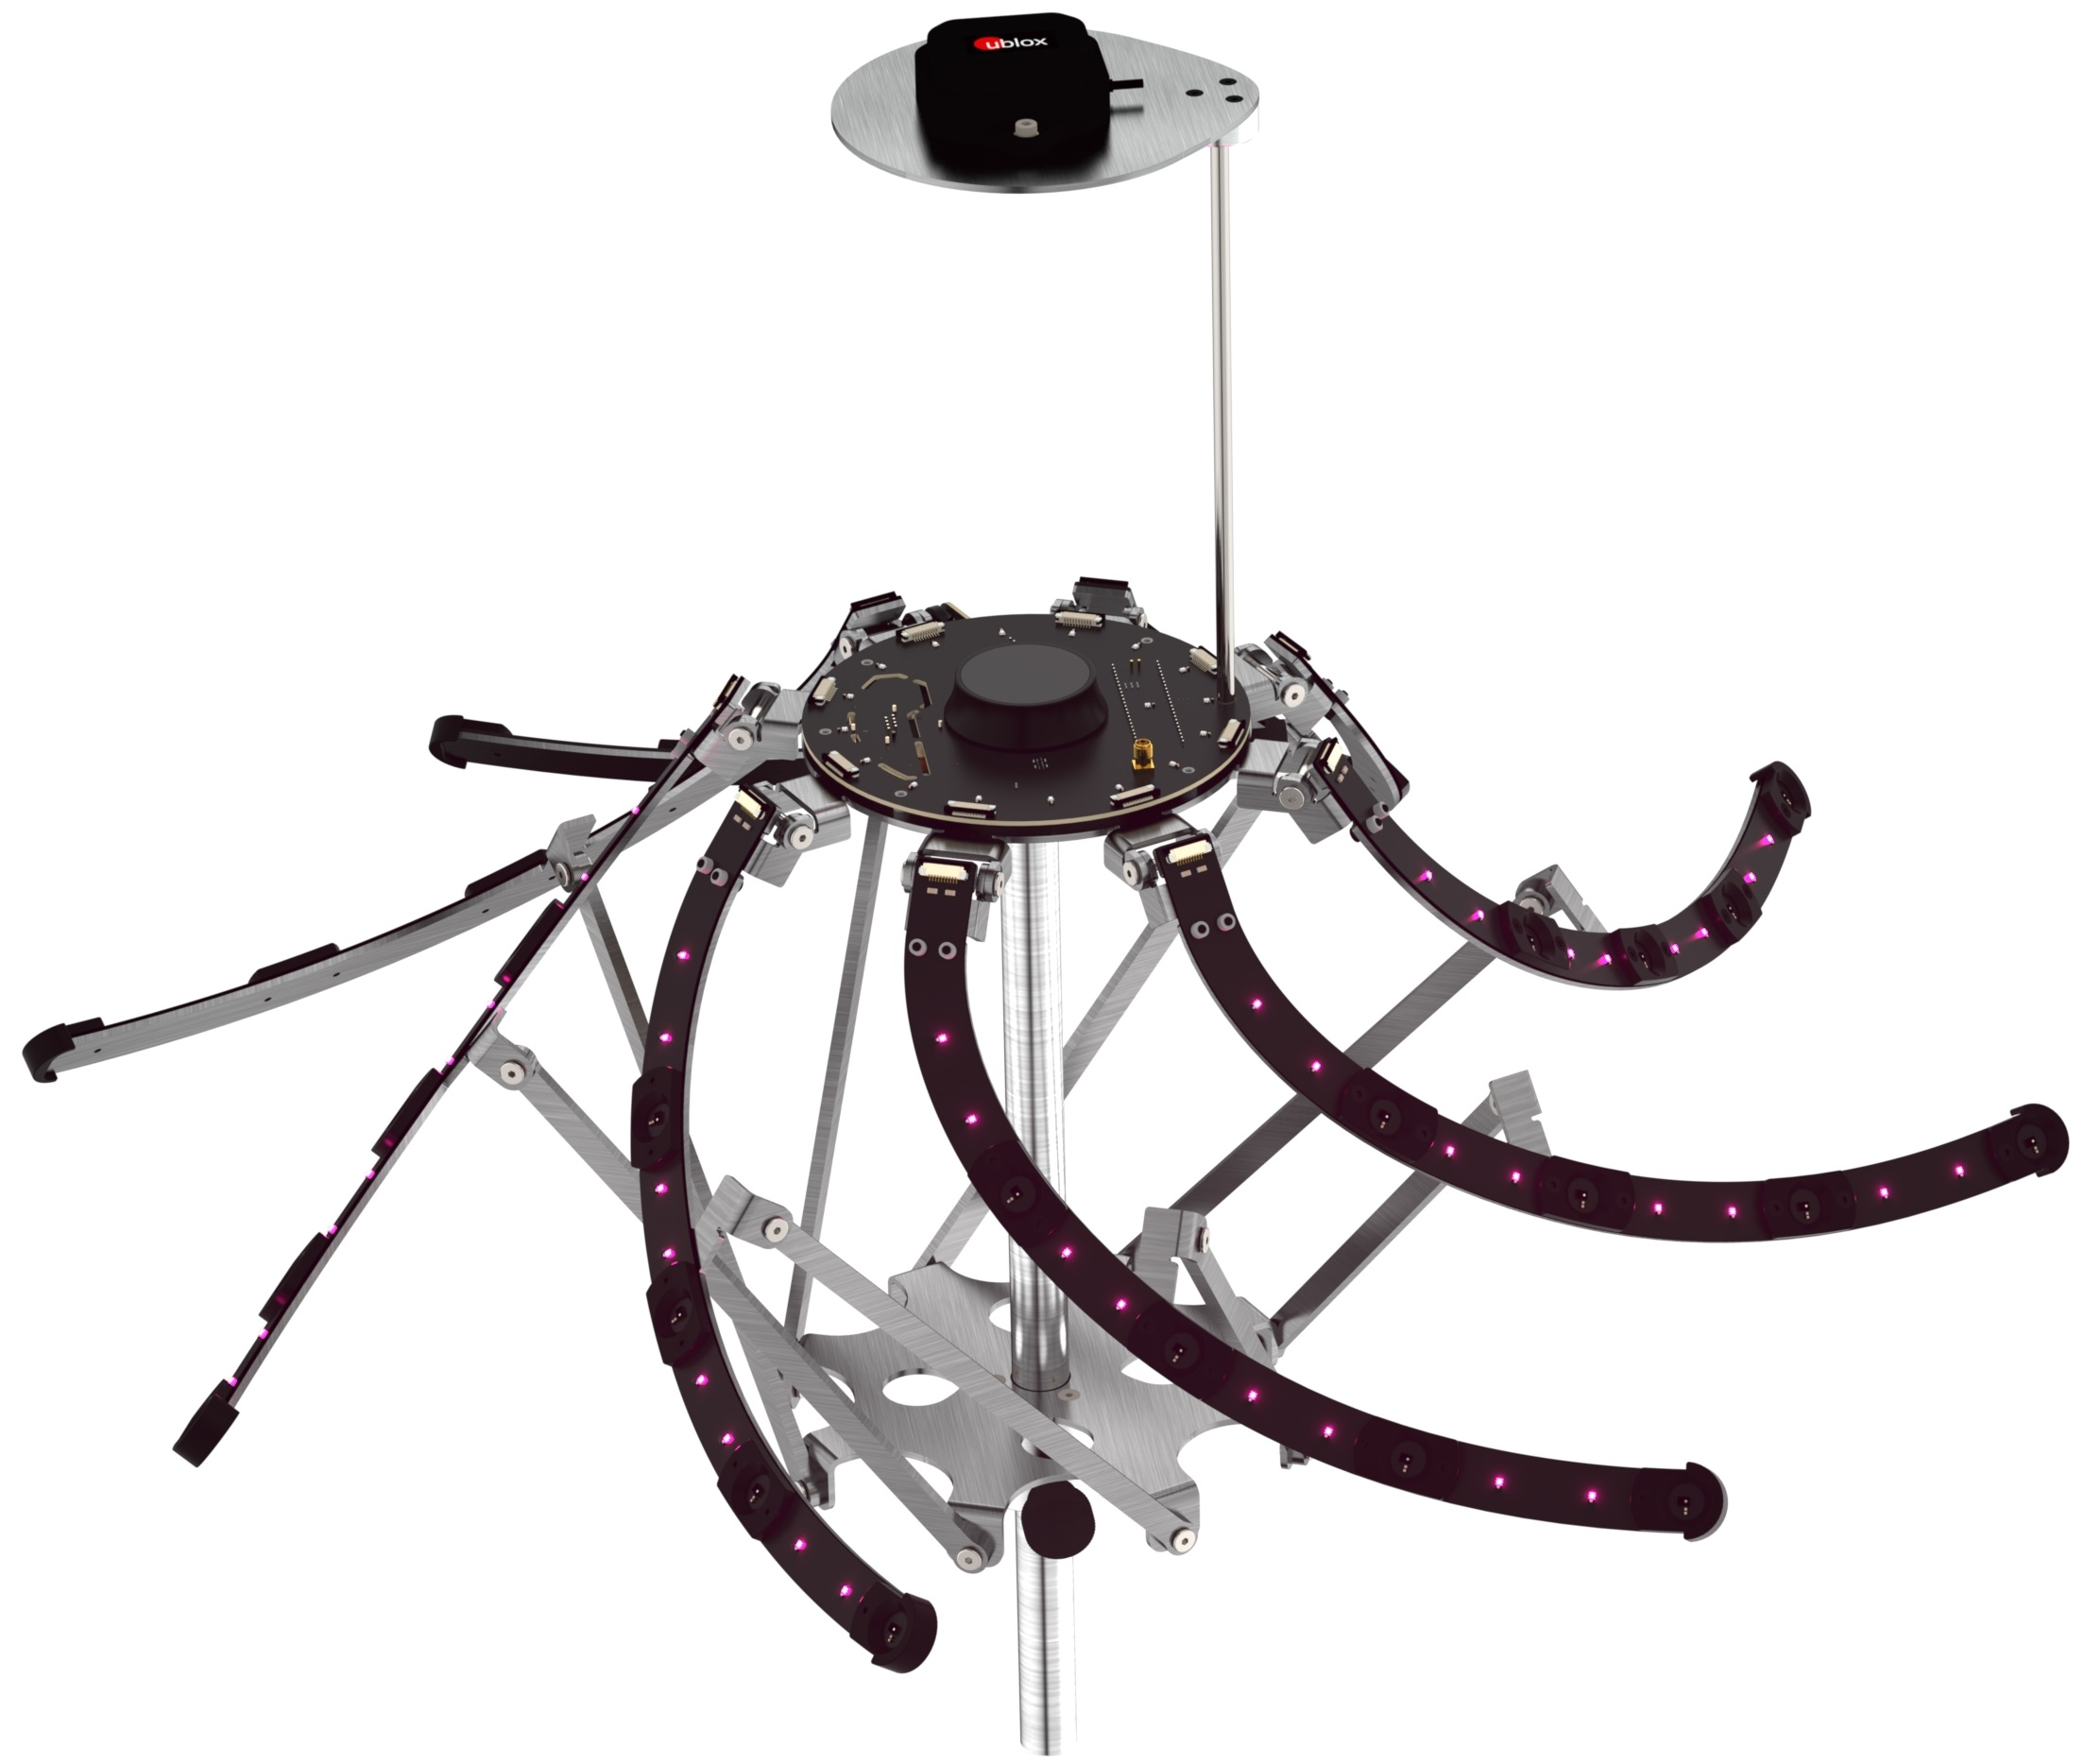
\includegraphics[width=1.0\textwidth]{images/6_design_final/final_design_3d_rendering.jpg}
	\caption{3D Rendering of the Final Design}
	\label{fig:final_design_3d_rendering}
\end{figure}
\pagebreak

\subsection{Part List}
The following list provides an overview of all custom manufactured metal parts:
\begin{itemize}
	\item 1x Top Mounting Platform: 2.5\,mm aluminum sheet metal
	\item 1x Bottom Sliding Platform: 2.5\,mm aluminum sheet metal
	\item 8x Microphone Arm Support Frame: 2.5\,mm aluminum sheet metal
	\item 8x Connection Bars: 5\,mm aluminum sheet metal
	\item 1x Antenna Platform: 2.5\,mm aluminum sheet metal
	\item 1x Main Mounting Pole: $\varnothing$\,20\,x\,400\,mm aluminum rod (Drawing: \ref{appendix_mechanical_drawing_main_mounting_pole})
	\item 1x Top Mounting Ring: $\varnothing$\,44\,x\,45\,mm aluminum part (Drawing: \ref{appendix_mechanical_drawing_top_mounting_ring})
	\item 1x Bottom Sliding Ring: $\varnothing$\,44\,x\,15\,mm aluminum part (Drawing: \ref{appendix_mechanical_drawing_bottom_sliding_ring})
	\item 1x Antenna Top Mount: $\varnothing$\,26\,mm\,x\,12\,mm aluminum part (Drawing: \ref{appendix_mechanical_drawing_antenna_top_mount})
	\item 1x Antenna Bottom Mount: 29.5\,x\,14.5\,x\,15.0\,mm aluminum part (Drawing: \ref{appendix_mechanical_drawing_antenna_bottom_mount})
	\item 1x Antenna Pole: $\varnothing$\,6\,x\,240\,mm stainless steel rod (Drawing: \ref{appendix_mechanical_drawing_antenna_pole})
\end{itemize}

\subsection{Microphone Arm Design}
Figure \ref{fig:mechanical_dimensions_microphone_arm} shows the mechanical dimensions of the microphone arm.
The pivot point is located at 95\,mm from the axial center of the microphone array.
Each microphone arm is oriented at an angle of 45\,° to the center pole.
\begin{figure}[h!]
	\centering
	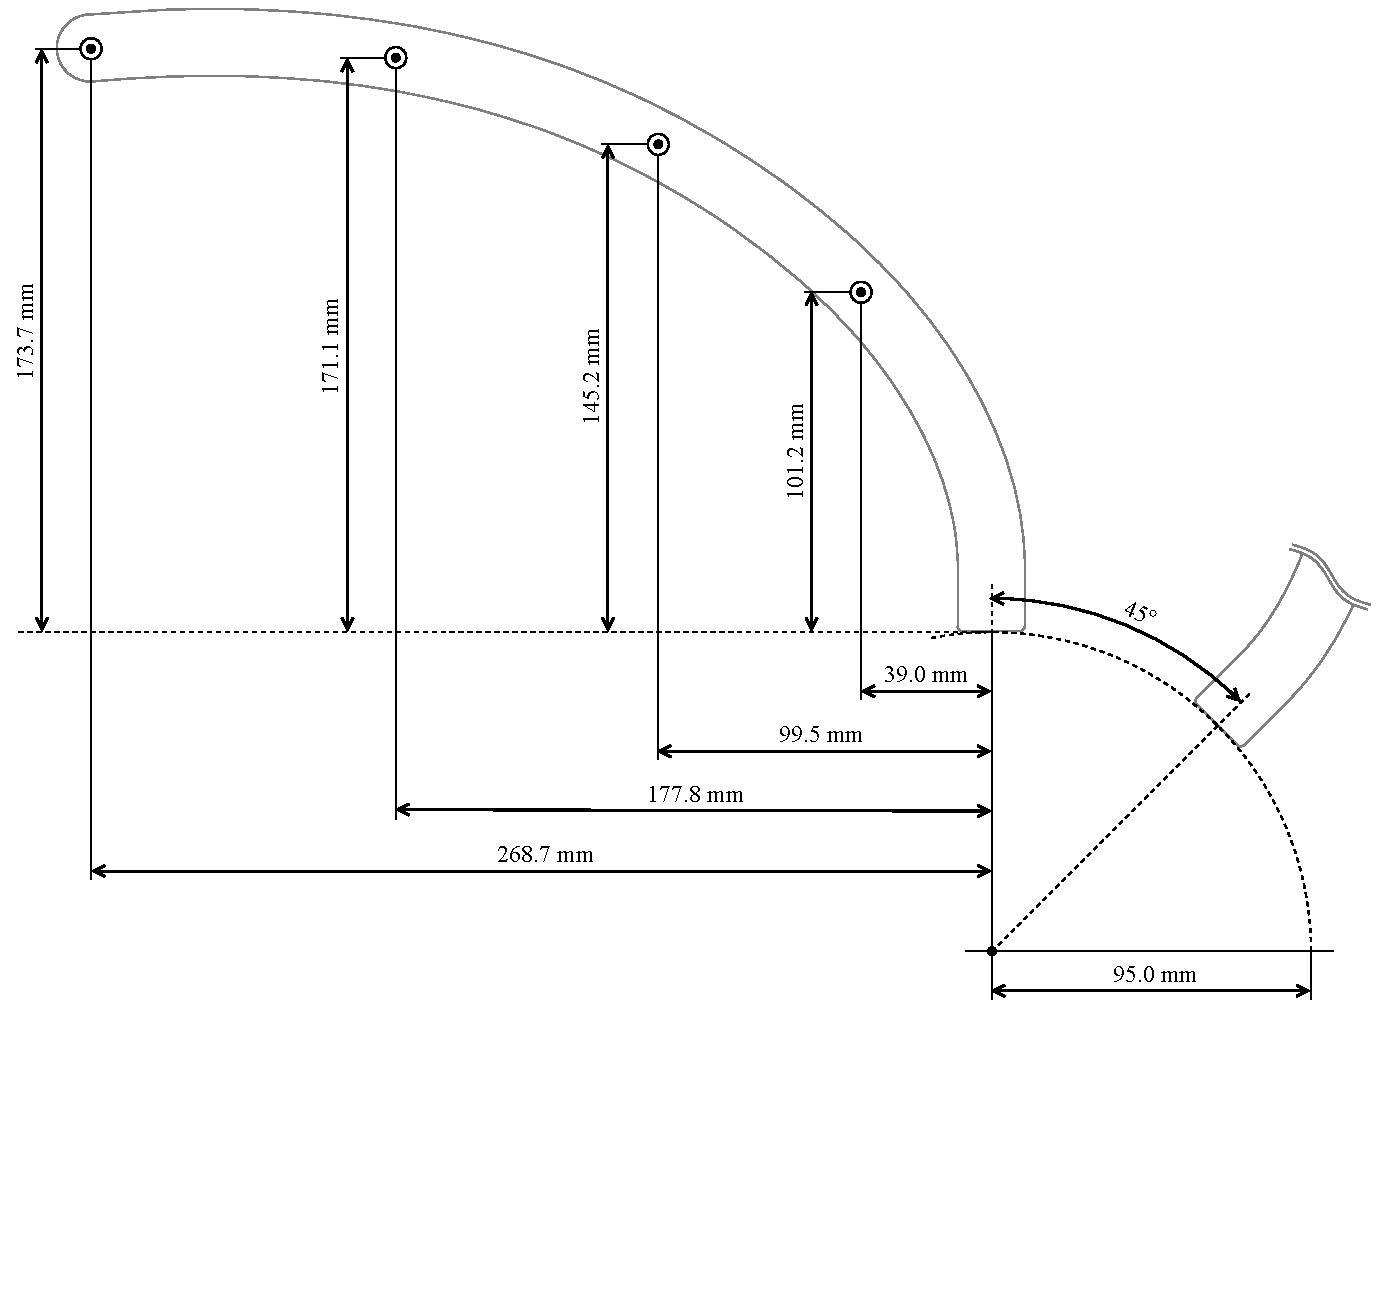
\includegraphics[width=1.0\textwidth, trim={0 4.9cm 0 0}]{images/6_design_final/array_final_design_mechanical_dimensions.pdf}
	\caption{Mechanical Dimensions of the Microphone Arm}
	\label{fig:mechanical_dimensions_microphone_arm}
\end{figure}
\pagebreak

\subsection{Folding Mechanism}
The microphone arms can be fully extended to achive a planar array geometry or folded towards the center pole to a minimum angle of 90\,°.
As figure \ref{fig:microphone_arm_folding_mechanism} shows, a cone shaped array structure results from this design.
The angle can be freely adjusted or locked in place using a M6 knurled screw located at the lower mounting platform.
\begin{figure}[h!]
	\centering
	\vspace{-0.1cm}
	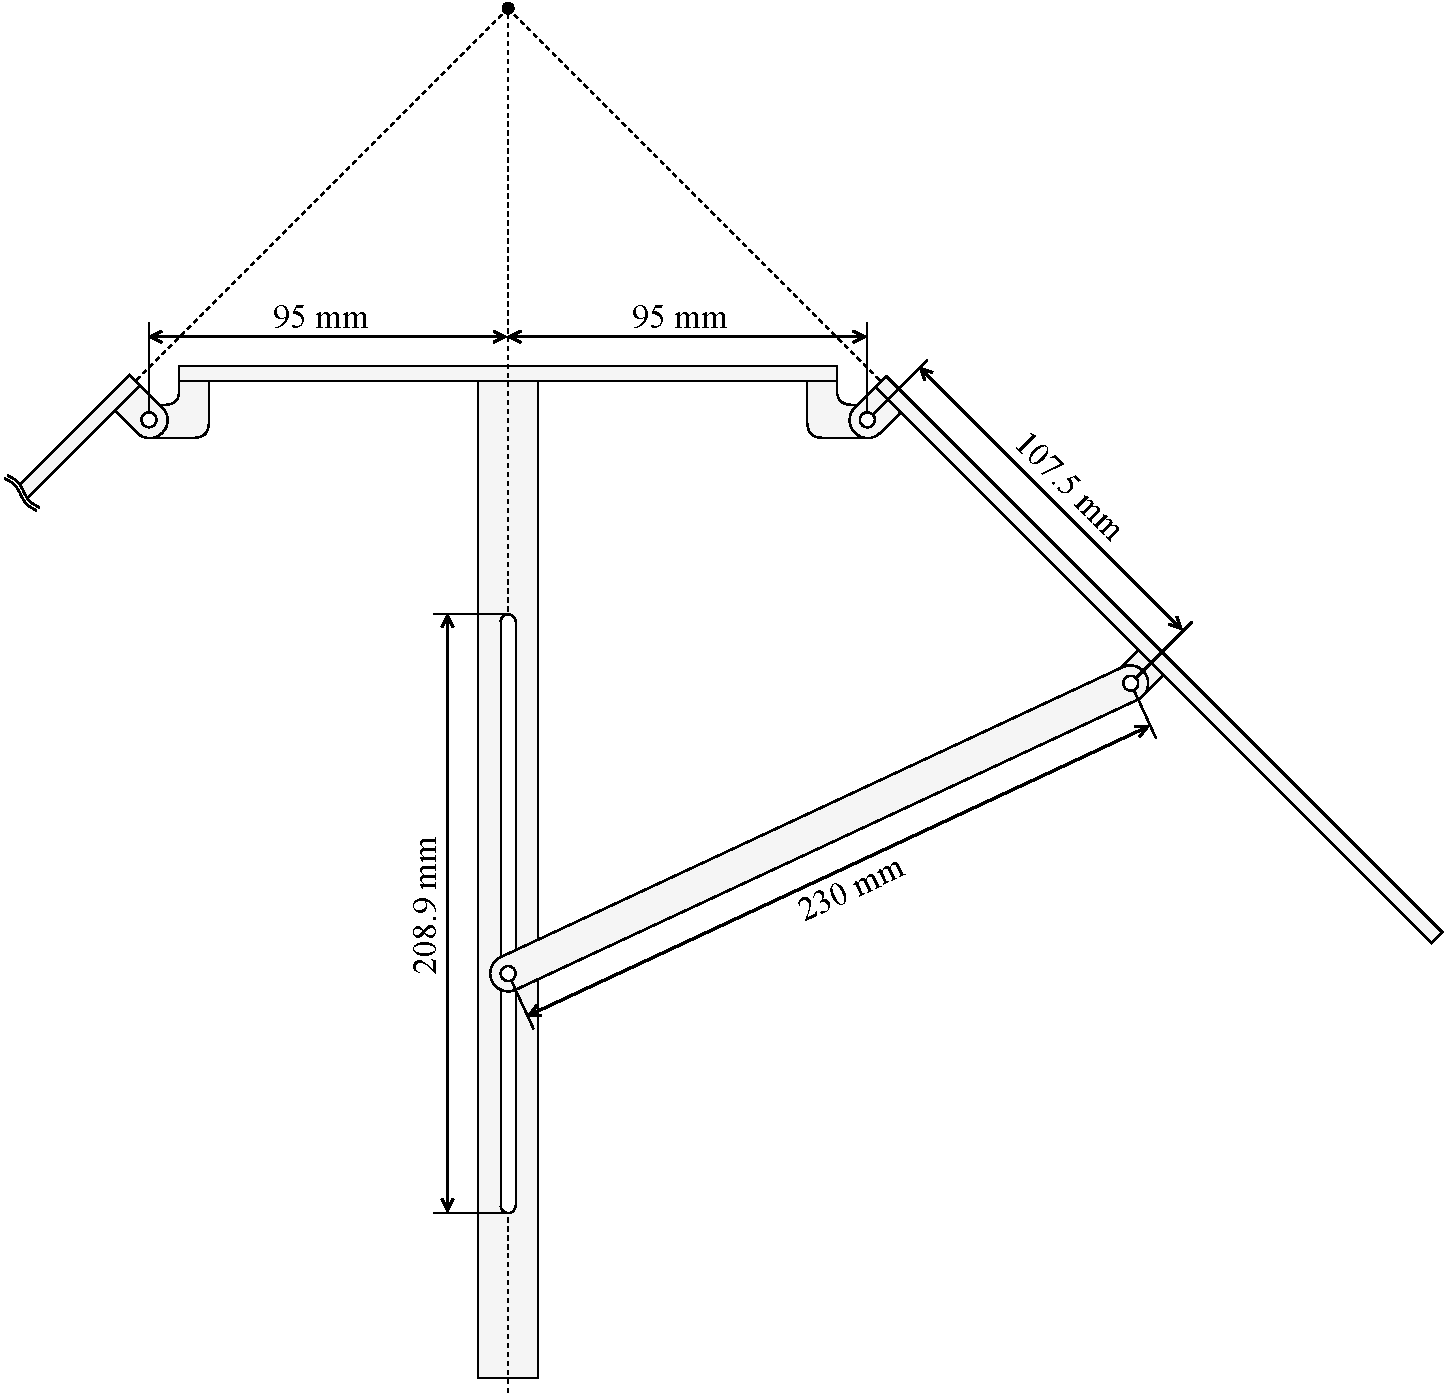
\includegraphics[width=0.84\textwidth]{images/6_design_final/microphone_arm_folding_mechanism.pdf}
	\hspace{-3.6cm}
	\caption{Mechanical Design of Folding Mechanism}
	\label{fig:microphone_arm_folding_mechanism}
\end{figure}

\subsection{Microphone Wind Protection}
As mentioned in section \ref{sec:array_prototype_measurements}, the microphone wind protection is a critical component of the design.
Therefor, each microphone is equipped with specialized microphone wind protection fur, which is attached to the microphone arm using a 3D-printed clip, as shown in figure \ref{fig:microphone_fur_clip_cad}.
\begin{figure}[h!]
	\centering
	\begin{minipage}{0.44\textwidth}
		\centering
		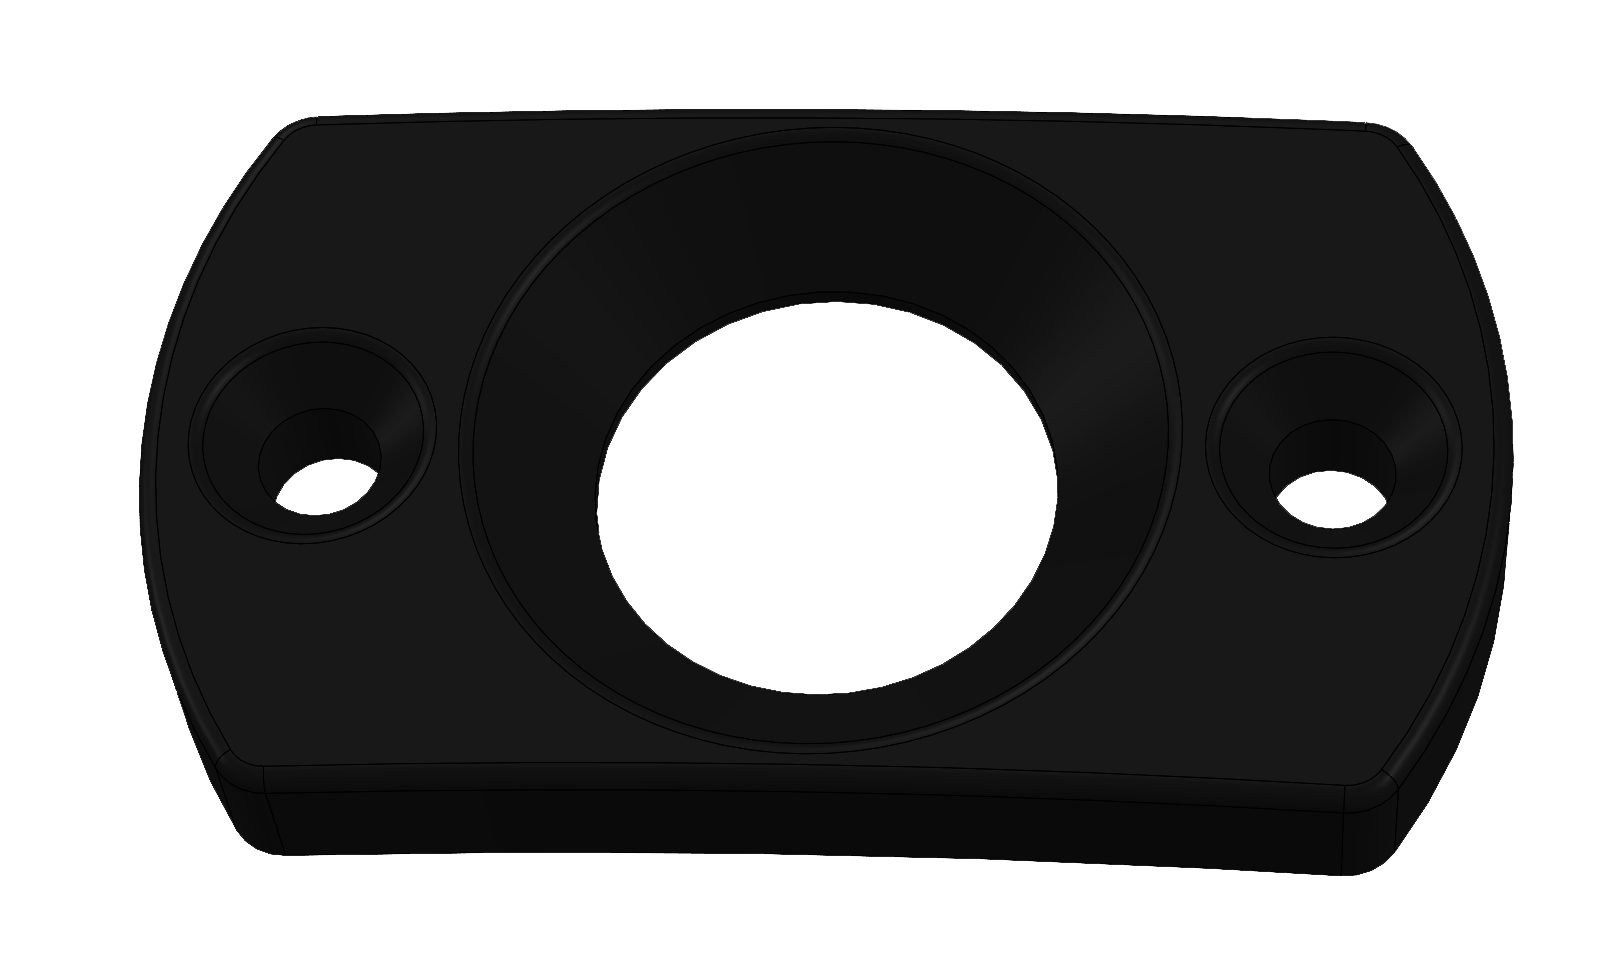
\includegraphics[height=3.3cm]{images/6_design_final/microphone_furr_clip_cad.png}
		\caption{3D-Printed Fur Clip}
		\label{fig:microphone_fur_clip_cad}
	\end{minipage}
	\begin{minipage}{0.55\textwidth}
		\centering
		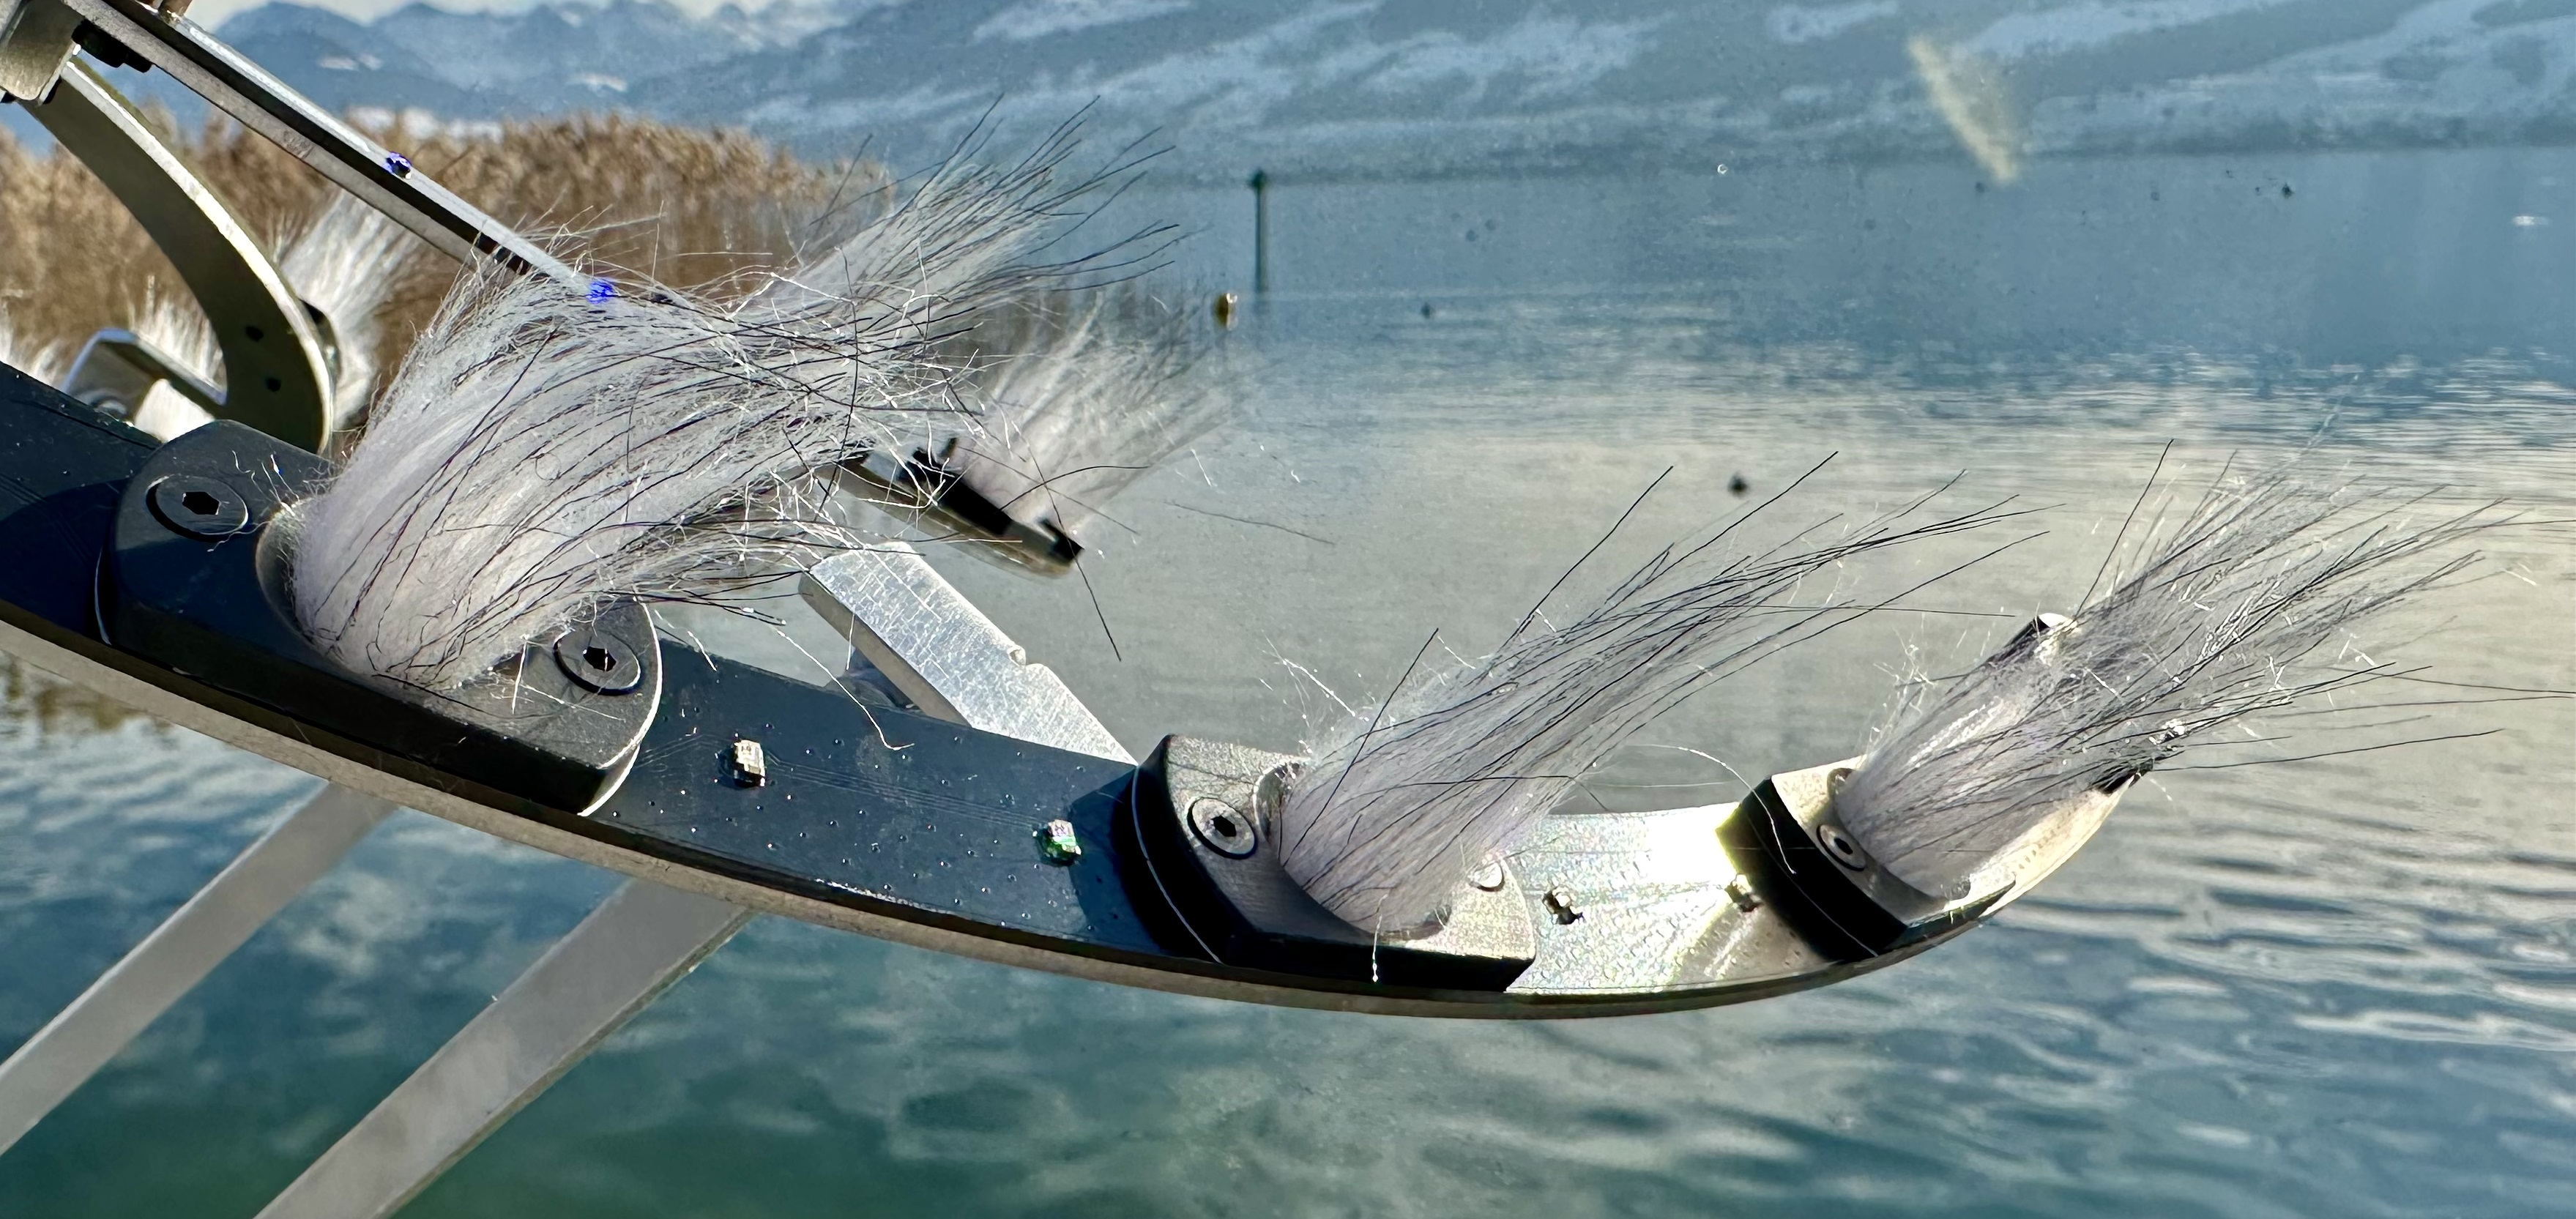
\includegraphics[height=3.3cm]{images/6_design_final/microphone_furr_clip.jpg}
		\caption{Microphone Wind Protection Fur}
		\label{fig:microphone_fur_clip}
	\end{minipage}
\end{figure}

\newpage
\section{Hardware Design}
The hardware design of the final sound source localization system is characterized by its multi-\acrshort{pcb} construction.
The system's central component is the mainboard, which houses the processing unit, various sensors, and the power supply.
In the center of the mainboard, a round touch display is mounted, which serves as the primary interface for user interaction.

Surrounding the mainboard are eight microphone arm \acrshort{pcb}s, each connected to the mainboard by 50\,mm long, 10-Pin flex-cables with a 1\,mm pin pitch.
These flex-cables provide the mechanical flexibility required adjusting the angle of the microphone arms.
Mounted on each microphone arm \acrshort{pcb} are four \acrshort{mems} microphones.
These microphones are strategically positioned as specified in section \ref{sec:final_array_geometry}.
Additionally, each arm is equipped with eight \acrshort{rgb} \acrshort{led}s, which serve both functional and aesthetic purposes, offering visual feedback and enhancing the system's overall design.
To accurately measure the angle of the microphone arms, a dedicated angle sensor \acrshort{pcb} was developed.

The entire hardware was designed using \textit{Altium Designer 23}, a leading software in \acrshort{pcb} design.
\begin{figure}[h!]
	\centering
	\vspace{0.3cm}
	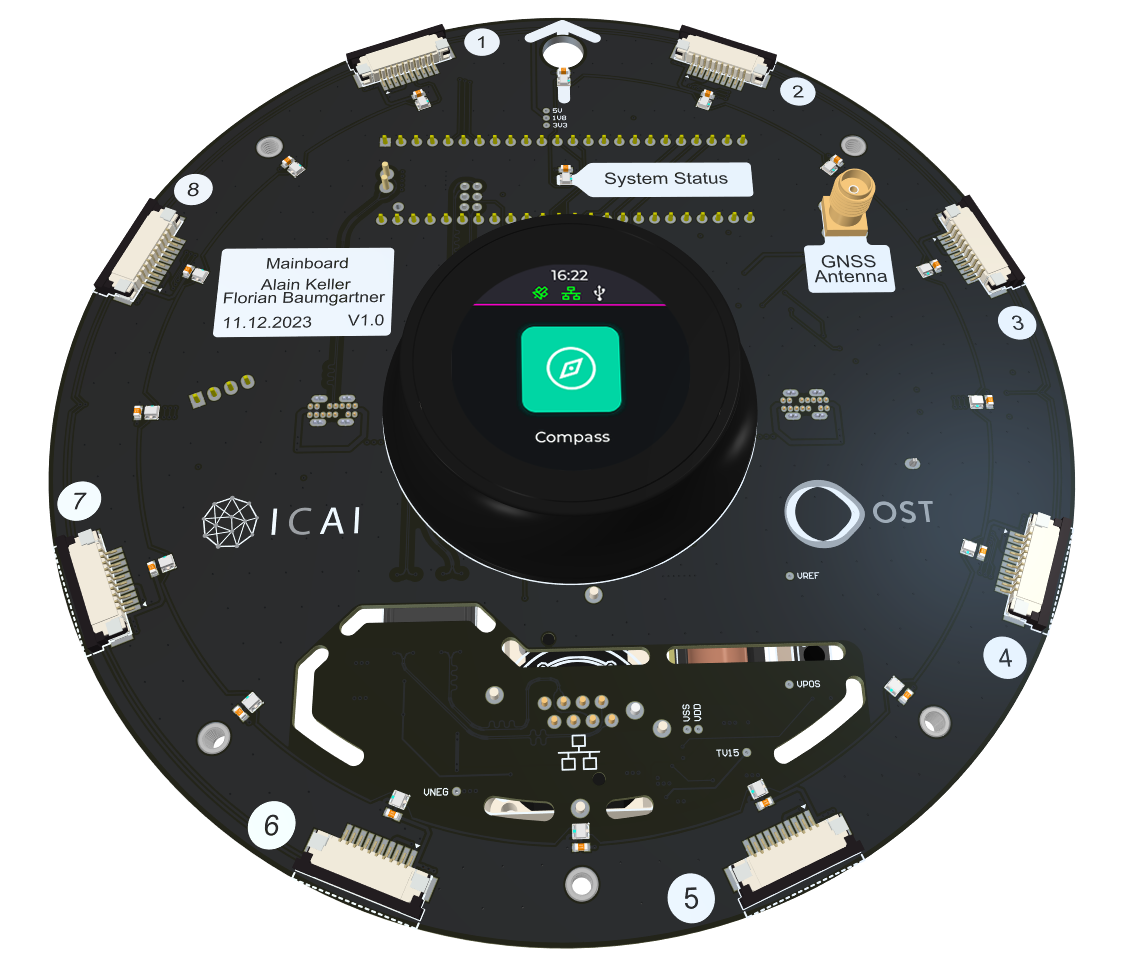
\includegraphics[width=1.0\textwidth]{images/6_design_final/Mainboard_Front_Display.png}
	\caption{Front View of the Mainboard}
	\label{fig:mainboard_front}
\end{figure}
\newpage

\subsection{Block Diagram}
The system block diagram in figure \ref{fig:system_block_diagram} provides an overview of the hardware design.
Note that components marked inside dashed boxes are located on separate \acrshort{pcb}s.
\begin{figure}[h!]
	\hspace{-1.3cm}
	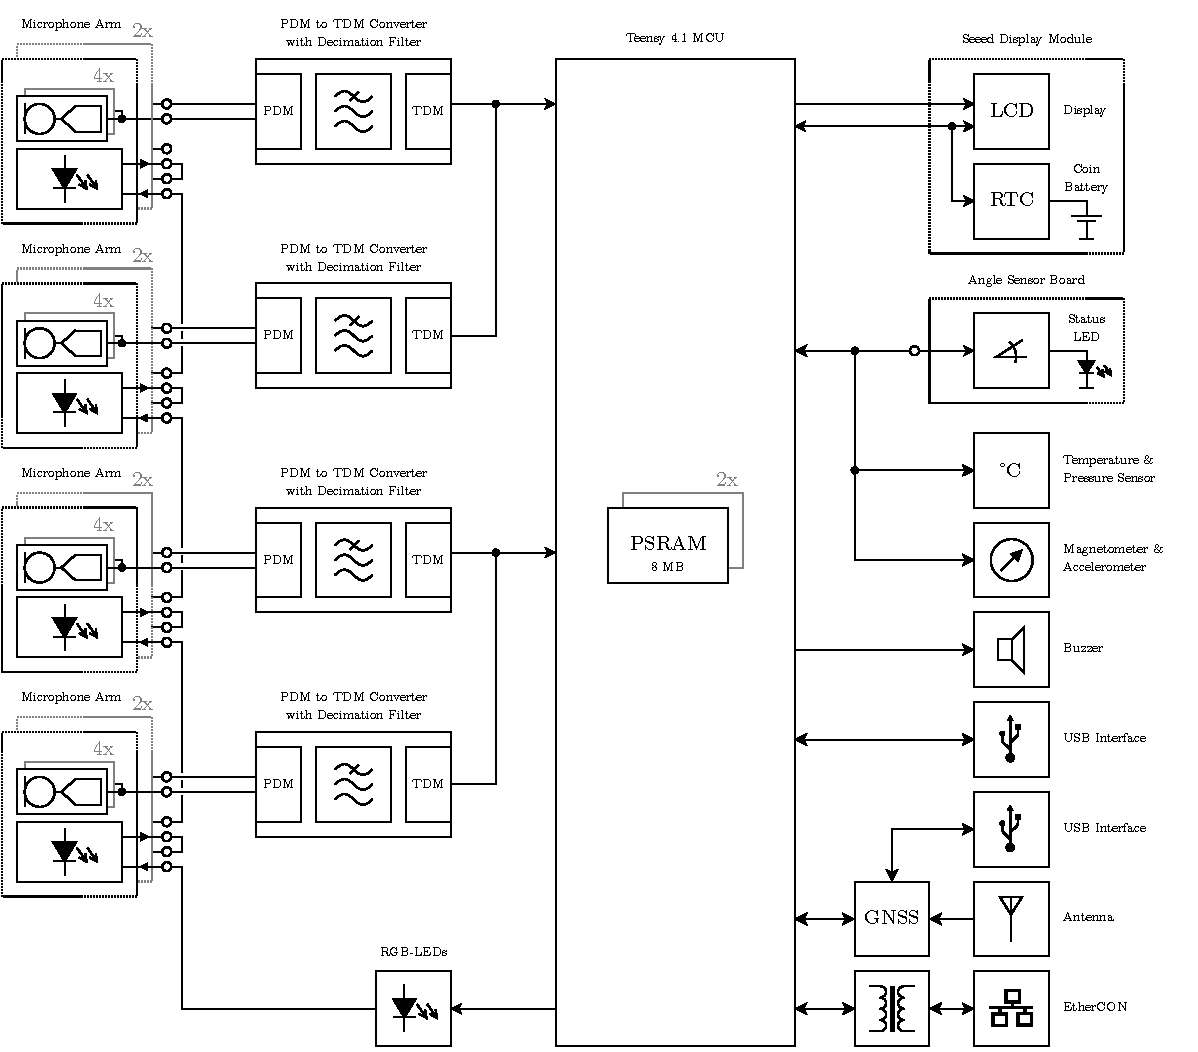
\includegraphics[width=1.28\textwidth, angle=90]{images/6_design_final/final_design_block_diagram.pdf}
	\vspace{-0.1cm}
	\caption{System Block Diagram}
	\label{fig:system_block_diagram}
\end{figure}
\newpage

\subsection{Power Supply}
The device can be powered by multiple sources.
Primary the device is powered by the ethernet interface, which provides a \acrfull{poe} connection.
This is the preferred method, as it is the most convenient way to use the microphone array in the field.
In addition, there are two \acrshort{usb}-C ports (\acrshort{mcu} and \acrshort{gnss}) that can be used to supply power when no \acrshort{poe} connection is available (e.g. in a laboratory environment for programming and debugging).
Each supply method can be used in conjunction with each other. However, the source must be able to provide at least 12.5\,W of power (5\,V, 2.5\,A).
In figure \ref{fig:power_supply_overview} an overview of the power supply is shown.
Note that the Teensy 4.1 has an internal 3.3\,V regulator, which is powered by the systems internal 5\,V supply.
The 1.8\,V rail is generated by a dedicated linear voltage regulator and is mainly used for the \acrshort{pdm} to \acrshort{tdm} converters (ADAU7118).
\begin{figure}[h!]
	\centering
	\vspace{-0.2cm}
	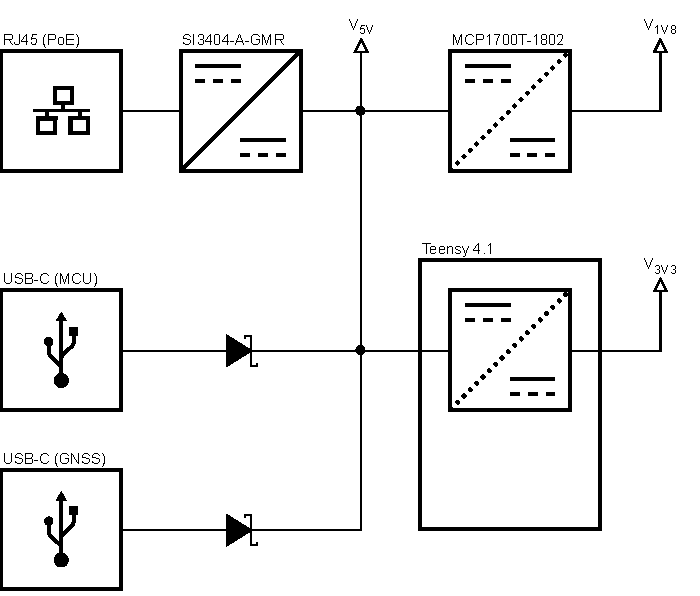
\includegraphics[width=0.65\textwidth]{images/6_design_final/final_design_power_supply.pdf}
	\vspace{-0.2cm}
	\caption{Power Supply Overview}
	\label{fig:power_supply_overview}
\end{figure}

\subsubsection{Power over Ethernet (PoE)}
For the power supply of the device, the \acrfull{poe} standard \acrshort{ieee}\,802.3at was implemented.
This standard allows for up to 12.95\,W of power to be delivered to the consumer side.
The system employs active \acrshort{poe}, necessitating the use of a negotiation \acrfull{ic}.
The \textit{SI3404} by \textit{Skyworks} was selected for this purpose, which, in addition to handling the communication protocol, incorporates a flyback step-down converter controller.

To adhere to \acrshort{poe} standards, it is mandatory for every power sink device to be galvanically isolated from the power sourcing equipment.
In this design, a transformer is used to step down the \acrshort{poe} voltage, typically around 56\,V, to the system voltage of 5\,V.
Furthermore, a second Ethernet signal transformer is employed to isolate the two data transmission pairs.
The total output power of the system is designed to be 2.5\,A at 5\,V.

For the Ethernet connection, the \textit{EtherCON} connector by \textit{Neutrik} was chosen.
This connector offers enhanced mechanical robustness compared to standard RJ45 connectors.
However, is is also compatible with standard RJ45 connectors.

\newpage
\subsection{Microcontroller Unit (MCU)}
As the main processing unit, the \textit{Teensy 4.1} was selected again, since it proved to fulfill all requirements.
However, during the firmware development, it became apparent that to meet the necessary ethernet throughput and internal processing power for the project,
the \textit{Teensy 4.1} had to be overclocked to 912\,MHz.
This increase in processing speed necessitated additional measures for thermal dissipation.
Consequently, a passive heatsink was mounted onto the \acrshort{soc} to effectively manage the increased heat generation.

Furthermore, the use of two external 8\,MB \acrshort{psram} chips was again deemed necessary.
These additional memory chips provide sufficient audio buffering capabilities,
essential for the system's performance in handling and processing the audio stream.

\subsection{Audio Input}
The audio input hardware builds upon the previous design detailed in section \ref{sec:acquisition_system_audio_input}, featuring four \textit{ADAU7118} \acrshort{pdm} to \acrshort{tdm} converters.
Two of these converters are connected to each \acrshort{tdm}-16 interface on the \textit{Teensy 4.1}.
Each converter \acrshort{ic} manages eight \acrshort{mems} microphones, effectively handling two microphone arms.

\subsection{GNSS Receiver}
The mainboard of the sound source localization system employs a \textit{NEO-M8P-2} module by \textit{uBlox} as its \acrshort{gnss} receiver,
chosen for its ease of integration into embedded systems through its versatile serial interfaces, including \acrshort{spi}, \acrshort{i2c}, \acrshort{uart}, and \acrshort{usb}.
For this specific application, the \acrshort{i2c} interface was utilized to connect the module to the \textit{Teensy\,4.1}.
Additionally, the module's \acrshort{usb} interface is extended to a dedicated \acrshort{usb}-C port, offering enhanced debugging capabilities with tools provided by \textit{uBlox}.

The design of the antenna frontend is tailored to drive active \acrshort{gnss} antennas, incorporating an inductor to couple the 3.3\,V supply voltage into the \acrshort{rf} line.
This setup powers the built-in \acrshort{lna} of the external antenna, ensuring optimal signal reception.
A standard \acrshort{sma} connector is used for connecting the antenna.

The module is also equipped with direct digital outputs for conveying status information.
A yellow \acrshort{led}, linked to the \acrshort{rtk}-Status output, illuminates to indicate when the module is in \acrshort{rtk} mode and has precisely determined its position.
Additionally, a red \acrshort{led} connected to the 1\,Hz time pulse output serves as an indicator, flashing briefly every second to signify a fixed \acrshort{gnss} status.

\subsubsection{External Antenna}
\begin{minipage}{\linewidth}
	\begin{wrapfigure}{r}{5.8cm}
		\vspace{-0.2cm}
		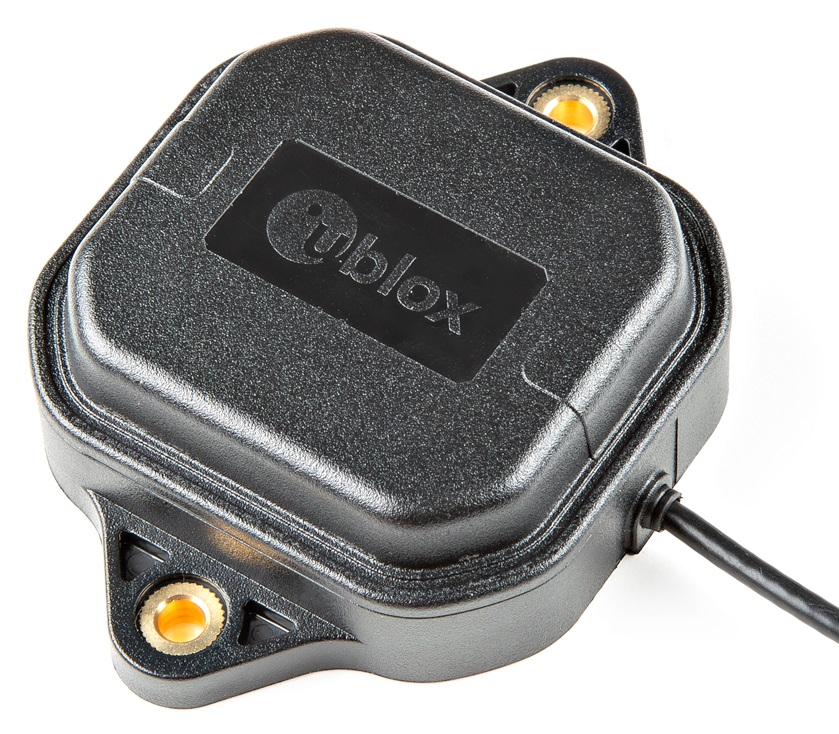
\includegraphics[width=5.3cm]{images/6_design_final/gnss_antenna.jpg}
		\centering
		\caption{GNSS Antenna (ANN-MB1-00)}
		\label{fig:gnss_antenna}
	\end{wrapfigure}
	The external \acrshort{gnss} antenna selected for this project is the \textit{ANN-MB1-00} from \textit{uBlox}.
	It supports both the L1 and L5 bands, making it versatile for various satellite systems including \acrshort{gps}, \acrshort{glonass}, Galileo, and BeiDou.
	The original 5\,m cable was shortened to approximately 30\,cm, and a new \acrshort{sma} connector was attached to the end.
	A crucial aspect of these multi-band antennas is their need for a metal base with a diameter of at least 10\,cm to enhance signal reception.
	To meet this requirement, the antenna is mounted on a dedicated aluminum platform, as shown in figure \ref{fig:final_design_3d_rendering}.
\end{minipage}
\newpage

\subsection{Display Module}
\begin{minipage}{\linewidth}
	\begin{wrapfigure}{r}{5.8cm}
		\vspace{-0.6cm}
		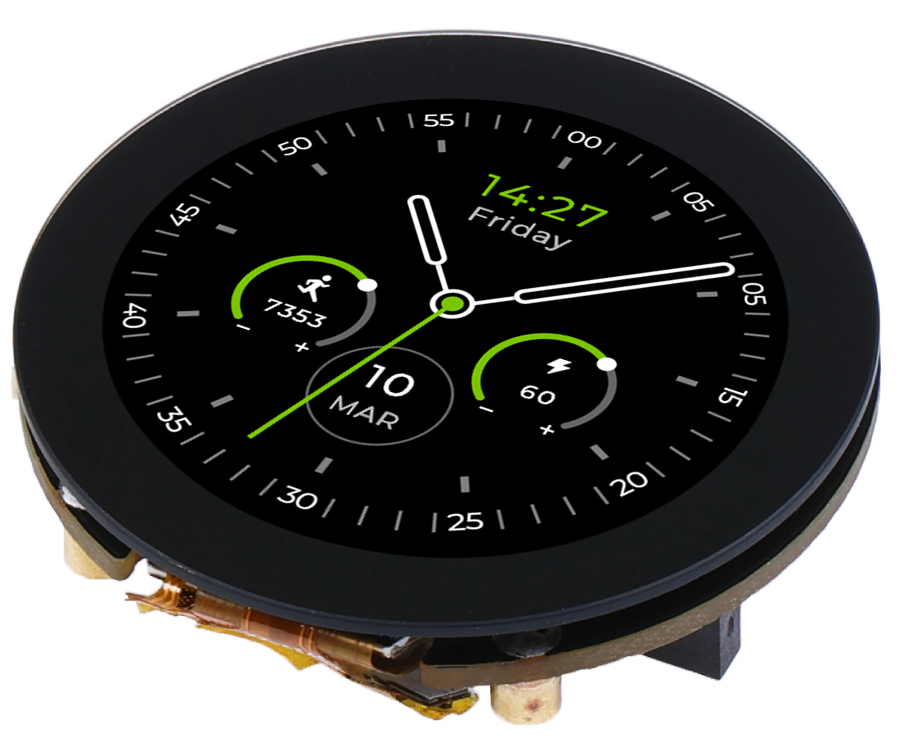
\includegraphics[width=5.3cm]{images/6_design_final/seeed_round_display_module.png}
		\centering
		\caption{Seeed Round Display Module}
		\label{fig:seeed_round_display_module}
	\end{wrapfigure}
	The display module, a round \acrshort{tft} unit from \textit{Seeed Electronics}, features a 240\,x\,240 pixel resolution and a 1.28\,inch (3.3\,cm) diameter.
	It operates via a high-speed \acrshort{spi} interface at 80\,MHz, allowing a smooth 30\,\acrshort{fps} refresh rate.
	Notably, the module includes an integrated \acrfull{rtc} of the type \textit{PCF8563},
	powered by a \textit{CR 927} (3\,V) coin cell battery, ensuring continuous timekeeping even when the main power is off.
	Additionally, the backlight brightness is adjustable via a \acrfull{pwm} output pin on the \textit{Teensy\,4.1}.

	Both the touchscreen and the \acrshort{rtc} are connected to the \textit{Teensy\,4.1} through the same \acrshort{i2c}.
	The module is mounted to the mainbaord with three M2 screws and a custom 3D-printed mounting ring.
\end{minipage}

\subsection{RGB LEDs}
In the sound source localization system, a total of 81 individually addressable \acrshort{rgb} \acrshort{led}s are utilized.
These \acrshort{led}s are of the type \textit{WS2812B-0807} and have a size of 2.0\,x\,1.8\,mm.
They feature a single wire data interface, which operates at 800\,kHz and are powered by the 5\,V supply.
However, due to the high potential power consumption when all \acrshort{led}s are set to full brightness (white), it is crucial to manage the power draw carefully.
The maximal power consumption of all \acrshort{led}s is approximately
\begin{equation} \label{eq:led_power_consumption}
	P_{\text{tot}} = V_{\text{sup}} \cdot N_{\text{LED}} \cdot I_{\text{max}} = 5\,\text{V} \cdot 81 \cdot 19\,\text{mA} \approx 7.7\,\text{W}.
\end{equation}
Consequently, the global brightness of the \acrshort{led}s must be limited through software.

\subsection{Sensors}
The mainboard of the sound source localization system is equipped with a variety of sensors.
Firstly, a combined magnetometer and accelerometer is implemented.
It provides crucial heading and leveling information for the device,
which is essential for providing accurate positioning information, specifically when utilizing multiple microphone arrays.

Additionally, the system incorporates a combined ambient pressure and temperature sensor.
This sensor plays a vital role in monitoring the ambient air conditions, a factor that significantly influences the accuracy of the beamforming algorithms used in sound localization.

Furthermore, a magnetic angle sensor is integrated into the design.
This sensor determines the current positions of the array arms.
Since all the arms are mechanically coupled and maintain the same angle relative to each other, only one of these angle sensors is required.

All sensors are connected to the \textit{Teensy 4.1} via a shared \acrshort{i2c} bus running at only 100\,kHz due to the relativly long physical distance between the sensors and the \acrshort{mcu}.
\newpage

\subsubsection{Magnetometer \& Accelerometer Sensor}
The \textit{LSM303AGRTR} by \textit{ST Microelectronics} was selected as the magnetometer and accelerometer, largely due to its wide availability, extensive software support, and high resolution.
This sensor uniquely combines a sensitive 3-axis magnetic flux measurement unit with a 3-axis \textit{LIS2MDL} accelerometer, providing comprehensive motion and orientation sensing capabilities.

A critical aspect of using any kind of magnetometer is the compensation of interference from ferromagnetic and paramagnetic materials.
This necessitates regular calibration of the sensor, especially when there are changes in the surrounding environment.
This calibration is essential to maintain the accuracy and reliability of the sensor's readings.
Detailed information and guidelines for the calibration process can be found in section \ref{sec:sensor_calibration}

\subsubsection{Ambient Pressure \& Temperature Sensor}
The \textit{BMP388} by \textit{Bosch Sensortec} was selected as the ambient pressure and temperature sensor.
This sensor has a pressure measurement range of 300\,-\,1250\,hPa, with an accuracy of ±\,8\,Pa ($\approx$\,0.66\,m) within the typical operating range of 900\,-\,1100\,hPa.
The integrated temperature sensor features a measurement accuracy of ±\,0.3\,°C in the range of 0\,-\,65\,°C.

During the \acrshort{pcb} design for the mainboard, however, the thermal placement of this sensor was not adequately considered.
Consequently, heat-emitting components on the board affect the \textit{BMP388}'s temperature readings, leading to a temperature offset of approximately 2.5\,°C.
A better approach would have been to isolate the sensor thermally, e.g. by creating a slot around the sensor on the \acrshort{pcb}.

\subsubsection{Angle Sensor}
The design utilizes the \textit{AS5600} magnetic angle sensor from \textit{AMS-Osram Semiconductors}.
This sensor offers 12-bit resolution and can accurately detect the position of a circular magnet, mounted at a distance of 0.5\,mm to 3\,mm.
Additionally, this sensor features a \acrshort{pwm} digital output, that has been connected to a dedicated \acrshort{led} on the angle sensor \acrshort{pcb}.
This \acrshort{led} provides a visual indication of the current angle being measured and confirms magnet detection.

Figure \ref{fig:angle_sensor_principle} shows the principle of operation of the \textit{AS5600} angle sensor.
\begin{figure}[h!]
	\centering
	\vspace{0.2cm}
	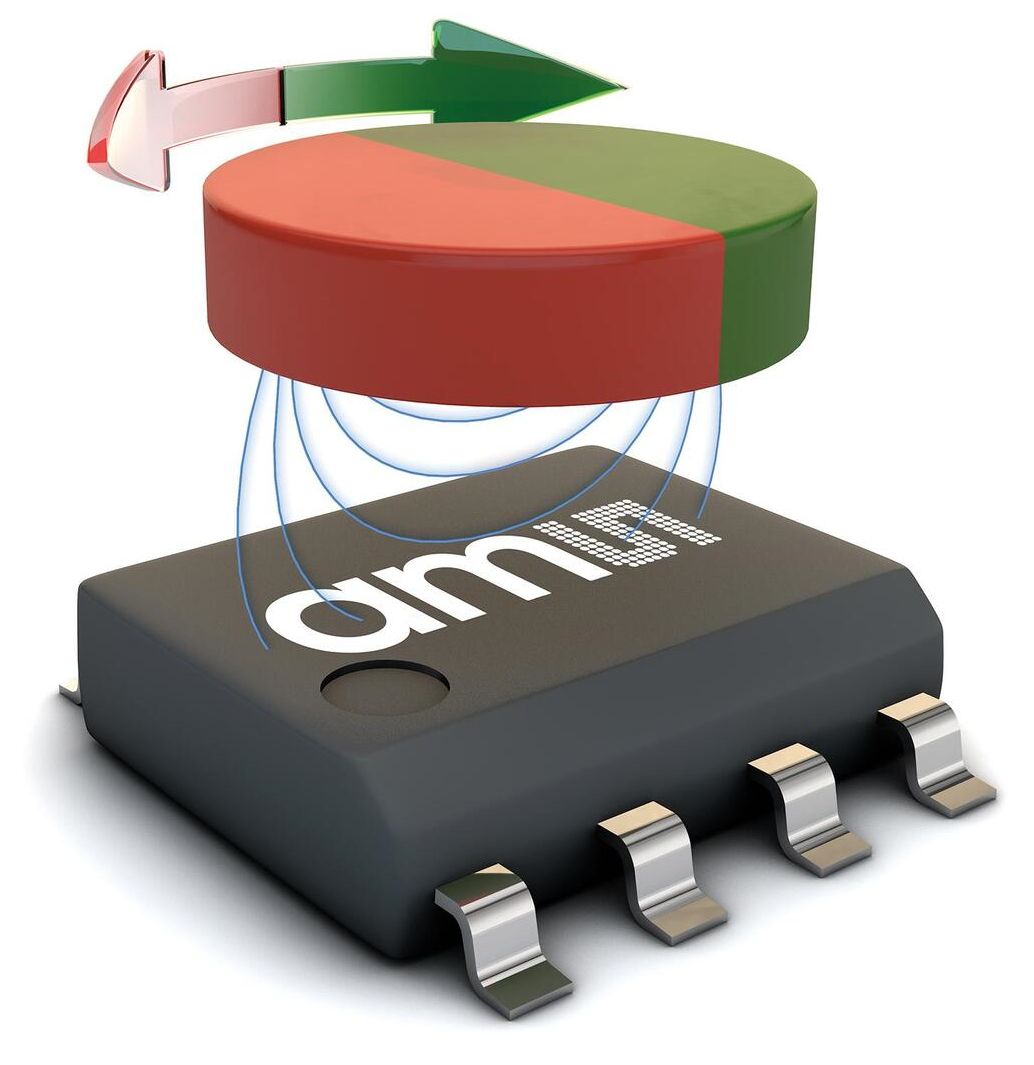
\includegraphics[width=4.8cm]{images/6_design_final/angle_sensor_principle.png}
	\caption{Operation Principle of the AS5600 Angle Sensor \cite{ams_osram_as5600}}
	\label{fig:angle_sensor_principle}
\end{figure}

\newpage
\subsection{Printed Circuit Boards (PCBs)}
The sound source localization system is based on three custom designed \acrshort{pcb}s.

\begin{minipage}{\linewidth}
	\begin{wrapfigure}{r}{7.0cm}
		\vspace{-0.1cm}
		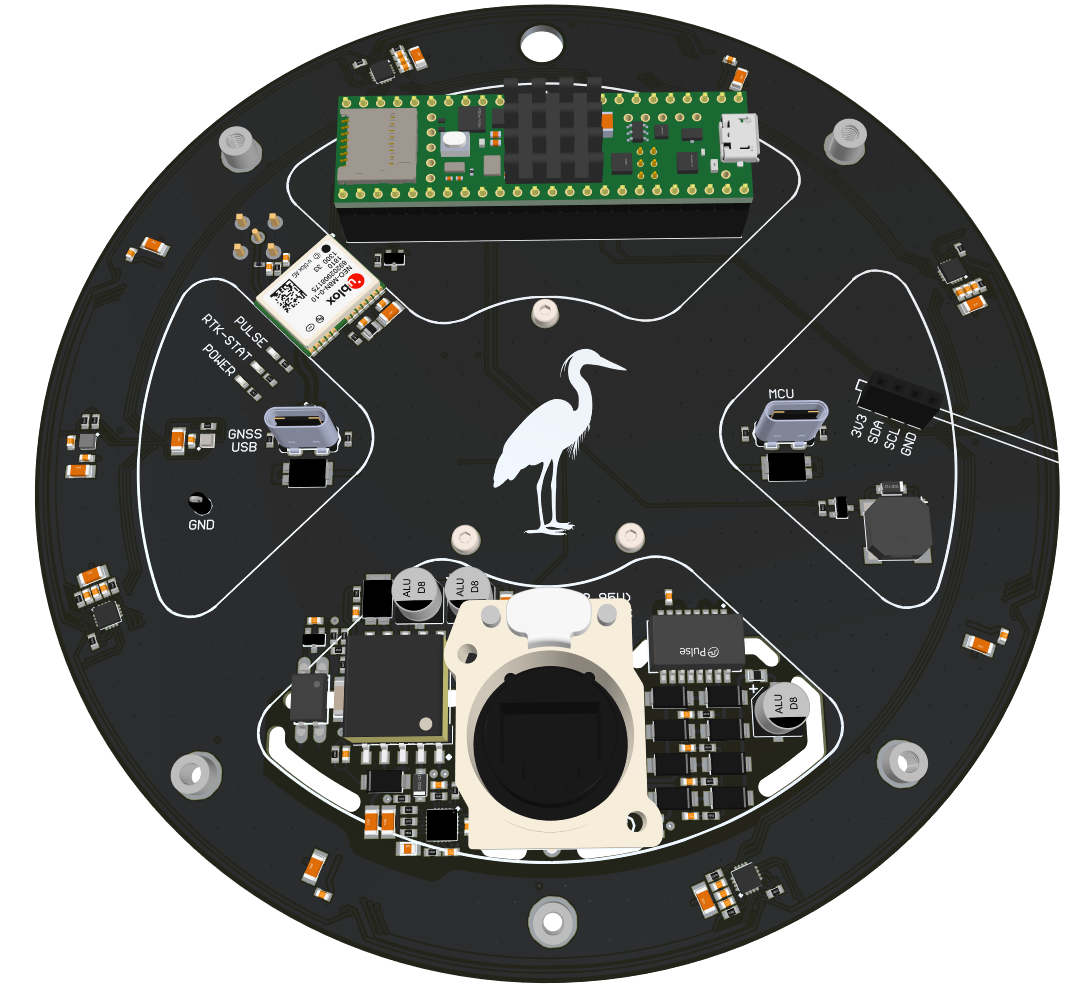
\includegraphics[width=6.5cm]{images/6_design_final/Mainboard_Back.png}
		\centering
		\caption{Mainbaord PCB}
		\label{fig:mainboard_pcb}
	\end{wrapfigure}
	\subsubsection{Mainboard}
	The Mainbaord is based on a 4-layer round \acrshort{pcb} with a diameter of 150\,mm.
	It utilizes a double-sided component assembly, primarily positioning elements on the \acrshort{pcb}'s underside, as detailed in the 3D visualization \ref{fig:mainboard_pcb}.
	A key design challenge involved accommodating components taller than 4\,mm.
	These had to be placed within the white-marked areas, corresponding to cutouts in the aluminum top mounting plate.
	The \acrshort{pcb} is securely mounted using five surface-mounted standoff M3 nuts.
\end{minipage}

\begin{minipage}{\linewidth}
	\begin{wrapfigure}{r}{7.0cm}
		\vspace{0.2cm}
		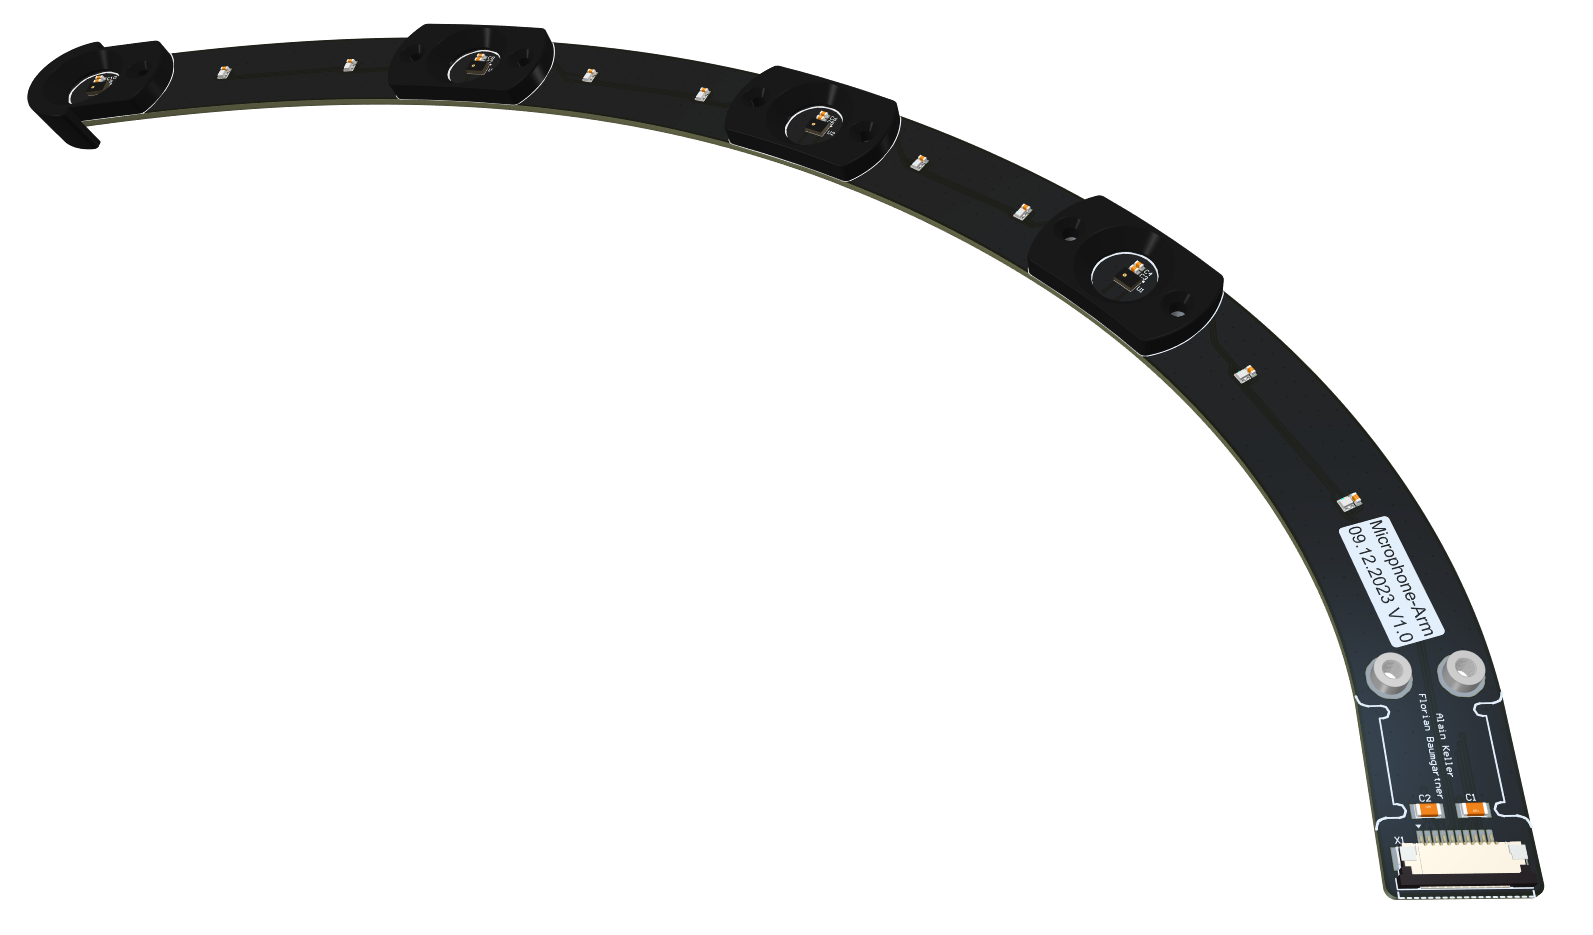
\includegraphics[width=6.5cm]{images/6_design_final/Microphone_Arm_Front.png}
		\centering
		\caption{Microphone Arm PCB}
		\label{fig:microphone_arm_pcb}
	\end{wrapfigure}
	\subsubsection{Microphone Arm}
	The Microphone Arm \acrshort{pcb} is a 2-layer design, measuring 288.7\,x\,190.4\,mm, with all components mounted on the top side.
	It features two surface-mounted M3 nuts near the connector side, which provide mechanical rigidity when mounted on the support frame.
	Additionally, the \acrshort{pcb} features seven 3.2\,mm mounting holes placed for attaching the microphone fur clips.
\end{minipage}

\begin{minipage}{\linewidth}
	\begin{wrapfigure}{r}{7.0cm}
		\vspace{0.2cm}
		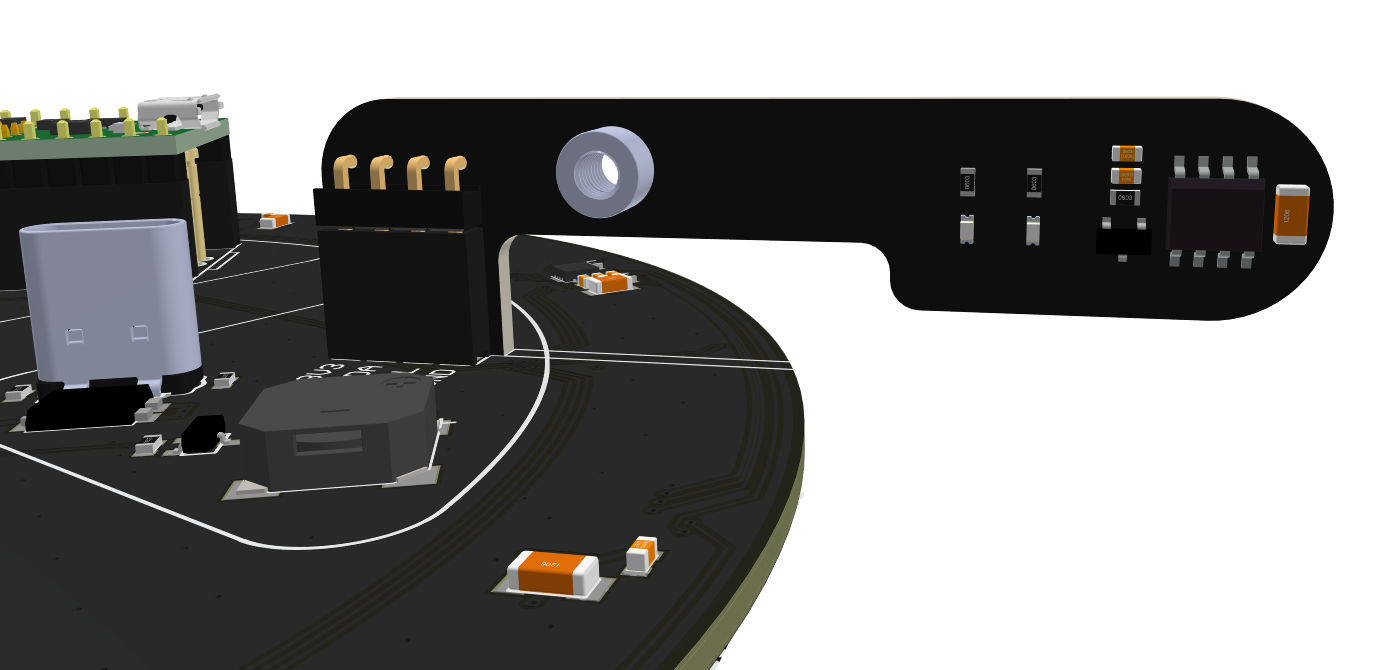
\includegraphics[width=6.5cm]{images/6_design_final/Angle_Sensor_Front.png}
		\centering
		\caption{Angle Sensor PCB}
		\label{fig:angle_sensor_pcb}
	\end{wrapfigure}
	\subsubsection{Angle Sensor}
	The Angle Sensor \acrshort{pcb} is a 2-layer design, measuring 61.25\,x\,16.5\,mm, with all components mounted on the bottom side.
	A standard 2.54\,mm pin header is used for connecting it to the mainboard.
	The magnetic angle sensor \acrshort{ic} is placed exactly at the pivot point of the microphone arm.
	The \acrshort{pcb} is mounted to the main frame using a 3D-printed fixture.
\end{minipage}

\subsection{Manufacturing}
The \acrshort{pcb}s were manufactured and assembled by \textit{JLCPCB}.
Only a few additional components were soldered by hand, such as the \acrshort{pdm} to \acrshort{tdm} converters (ADAU7118), the EtherCON connector and the \acrshort{gnss} module (NEO-M8P-2).
It turned out that multiple microphone arm \acrshort{pcb}s were faulty (damaged microphones).
This was most likely caused by the soldering process, as the \acrshort{mems} microphones are very sensitive to heat.

\newpage
\section{Firmware Design}
The firmware of the sound source localization system is build upon the audio acquisition system firmware.
It runs again on the \textit{Teensy 4.1} \acrshort{mcu} and the same toolchain has been used as described in section \ref{sec:acquisition_system_firmware_design}.
One of the main components of the firmware is the integration of the \textit{QNEthernet} stack.
However, integrating it proved to be quite challenging.
The \textit{QNEthernet} stack is not designed for a multithreaded environment, necessitating the main ethernet handler to operate in the main thread, i.e., the background thread.

\subsection{Overview}
The firmware is structured into multiple software modules, most of them running in their own thread.
Careful balancing of the thread priorities was essential to ensure the system's stability and performance.
Especially, enough processing headroom for the background thread had to be reserved, for high ethernet throughput and a fluent display refresh rate.
Table \ref{tab:threads} provides an overview of all threads and their purpose.
\begin{table}[h]
	\centering
	\begin{tabular}{|l|l|}
		\hline
		Thread                     & Purpose                      \\ \hline
		\texttt{Console Interface} & Handles USB virtual COM-Port \\ \hline
		\texttt{Console Streaming} & Handles queuing of messages  \\ \hline
		\texttt{Utils}             & Updates operation time       \\ \hline
		\texttt{AudioUtils}        & Audio Processing             \\ \hline
		\texttt{GNSS}              & GNSS Data Handling           \\ \hline
		\texttt{HMI}               & LED Control \& RTC           \\ \hline
		\texttt{Buzzer}            & Buzzer Control               \\ \hline
		\texttt{Application}       & Main Application Logic       \\ \hline
		\texttt{Main}              & Main Thread (Background)     \\ \hline
	\end{tabular}
	\caption{Overview of all Threads and their Purpose}
	\label{tab:threads}
\end{table}

\subsection{Audio Streaming}
The audio streaming module handles the buffering and transmission of the 32 audio channels.
It is based on a \acrshort{tcp} server that provides a socket connection on port 6666.
The audio data is transmitted in a lossless 16-bit signed integer format, with a sample rate of 44.1\,kHz.

The \acrshort{tcp} connection asures a reliable data transmission, which is essential for a continuous audio stream.
To ensure low latency, the audio data is buffered in a circular buffer of 12\,MB size.
This allows a maximal buffering time of approximately 4.4\,s.
A minimal tranmission rate of
\begin{equation}
	\frac{32\,\text{channels} \cdot 16\,\text{bit} \cdot 44100\,\text{Hz}}{10^6\,\text{bit/s}} = 22.1184\,\text{Mbit/s}
\end{equation}
is required.
The theoretical maximum transmission rate of 100Base-T Ethernet is 100\,Mbit/s.
However, the real-world tests with the \textit{Teensy 4.1} showed a maximum transmission rate of around 60\,Mbit/s, which is still sufficient for the audio stream.

\newpage
Due to the maximal \acrshort{tcp} packet size of 1460 bytes, the audio data is split into concatenated packets.
A frame consists of 128 interleafed samples (32 channels) and is transmitted in 8 packets.
Each frame starts with a 20-byte header, beginning with a magic sequence that allows the receiver to synchronize the incoming data stream.
Next is the packet index, which is incremented for each frame and enables the receiver to detect missing packets.
The last field is the timestamp in the \acrshort{unix} epoch format in nanoseconds.
Table \ref{tab:packet_header} shows the structure of the packet header.
\begin{table}[h!]
	\centering
	\begin{tabular}{|l|l|l|l|}
		\hline
		\textbf{Byte Offset} & \textbf{Data Format}    & \textbf{Description} & \textbf{Example Value} \\ \hline
		0-7                  & String                  & Magic Sequence       & \codeword{HERON666}    \\ \hline
		8-11                 & Integer (Little Endian) & Packet Index         & 12345                  \\ \hline
		12-19                & Integer (Little Endian) & Timestamp (ns)       & 1713586842696942069    \\ \hline
	\end{tabular}
	\caption{Description of the 20-byte Packet Header}
	\label{tab:packet_header}
\end{table}

Figure \ref{fig:frame_example} shows an example of a transmission sequence.
Note the interleafed sample order, which is based on the WAV file format.
\begin{figure}[h]
	\centering
	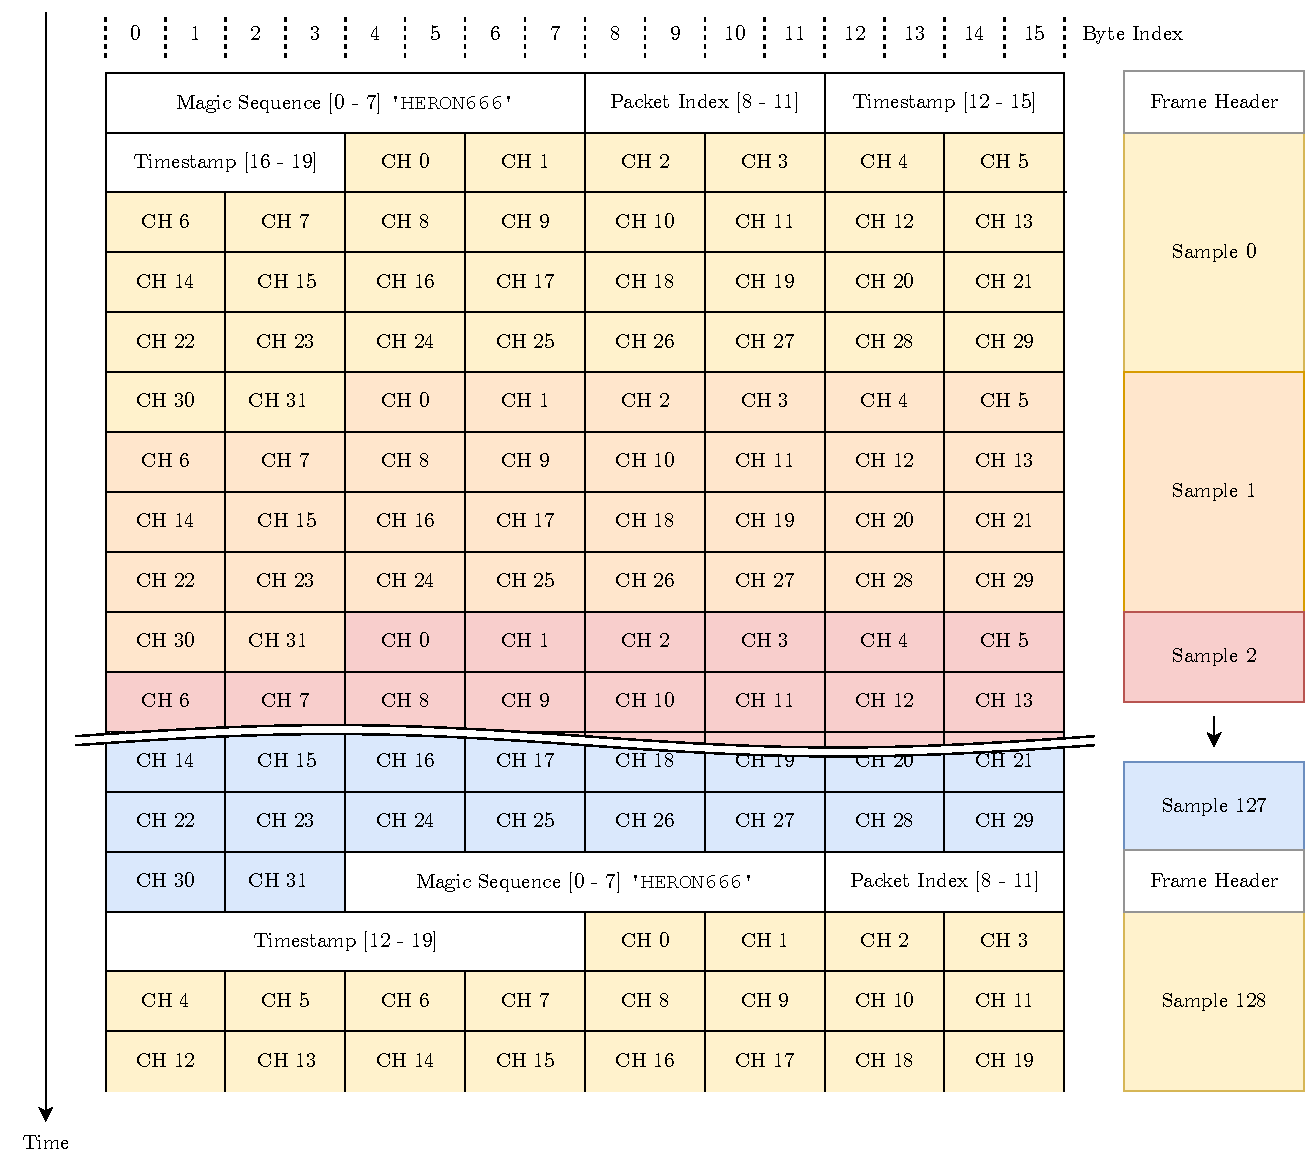
\includegraphics[width=1.0\textwidth]{images/6_design_final/Audio_Stream_Frame.pdf}
	\caption{Example of a Frame with 128 Samples (32 Channels)}
	\label{fig:frame_example}
\end{figure}

\newpage
\subsection{GNSS \& RTC Time}
The system incorporates two methods for timekeeping: A \acrshort{gnss} module and a \acrfull{rtc}.
The \acrshort{gnss} module is highly accurate, providing time information down to the nanosecond, which is essential for providing accurate timestamps for the audio stream.
In contrast, the \acrshort{rtc} is designed to maintain time even if the device loses power.
Once the \acrshort{gnss} time is established and stable, it automatically synchronizes the \acrshort{rtc}.
The \acrshort{gnss} module sends periodically its timing information to the \acrshort{mcu} at a rate of 5\,Hz.
Whenever a new time packet is received, the system logs the current internal system time in microseconds.
This allows calculating the time offset to any subsequent \acrshort{api} call which asks for the current time.

In situations where \acrshort{gnss} data isn't available, the system falls back to the \acrshort{rtc} time.
While this ensures continuous timekeeping, the \acrshort{rtc}'s limitation to second-level resolution presents a challenge.
It doesn't provide detailed information about the exact moment whenever a second has passed.
To address this and achieve more precise timing information, a specific algorithm is required as described in the following section.

\subsubsection{Phased Locked Loop (PLL)}
To estimate the subseconds of the current \acrshort{rtc} time, a \acrfull{pll} has been used in combination with a \acrshort{pi}-controller.
This approach effectively smooths out the \acrshort{rtc}'s stair-step signal, enhancing time resolution.
The Proportional (P) component of the \acrshort{pi}-controller is set to zero to avoid amplifying the \acrshort{rtc}'s abrupt second changes.
Instead, the focus is set on the Integral (I) component, which has been tuned by simulating the \acrshort{rtc}'s behavior in \textit{Python}.
In practice, an integral gain of 0.01 was found to provide best results.
The \acrshort{pll} algorithm is executed 5 times per second and can be described as
\begin{equation}
	\begin{aligned}
		t_{\text{PLL}}
		 & =
		t_{\text{SYS}} - t_\Delta  + 0.5\,\text{s} \\
		t_\Delta
		 & =
		K_p \cdot e + K_i \cdot \sum e             \\
		e
		 & =
		t_{\text{SYS}} - (t_{\text{RTC}} + t_\Delta) \;.
	\end{aligned}
\end{equation}
Figure \ref{fig:pll_measured_data} shows the measured timing data of the \acrshort{rtc} and the \acrshort{pll} output.
It can clearly be seen that the \acrshort{pll} output is approaching the interpolated \acrshort{rtc} time.
\begin{figure}[h]
	\centering
	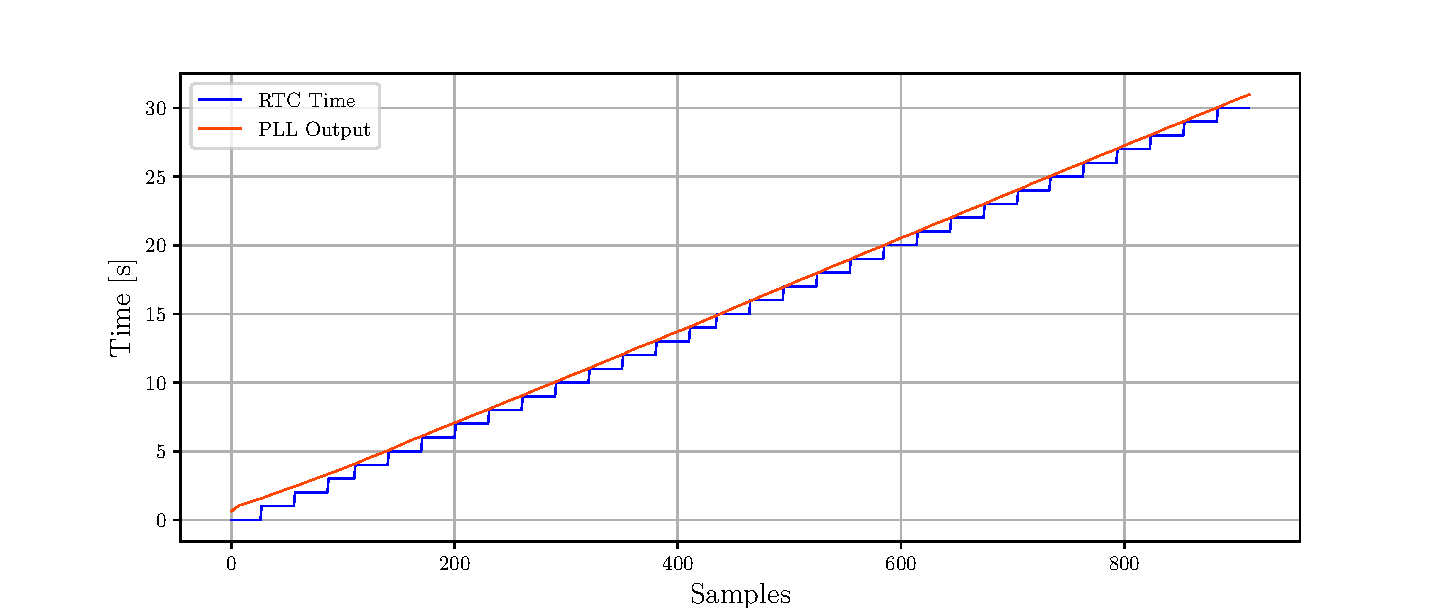
\includegraphics[width=1.0\textwidth]{images/6_design_final/PLL_Measured_Data_plot.pdf}
	\caption{Measured Timing Data of the RTC and PLL Output}
	\label{fig:pll_measured_data}
\end{figure}

\subsection{Remote Configuration}
The firmware includes an \acrshort{http} server on port 6667 that offers access to a \acrshort{json} file containing key system information.
This file, essential for remote management, details parameters such as the device's position, orientation, and status.
To retrieve this \acrshort{json} file, a simple \acrshort{http} GET request is made to the server's root \acrshort{url}.
This should be done periodically to ensure the most up-to-date information.
Table \ref{table:device_data_types} provides an overview of all data fields and their purpose.
\begin{table}[h!]
	\centering
	\tiny
	\begin{tabular}{|l|l|l|l|l|}
		\hline
		\textbf{Data Field}         & \textbf{Description}        & \textbf{Data Type} & \textbf{Unit} & \textbf{Example Value}       \\ \hline
		device\_firmware\_version   & Firmware Version            & String             & -             & \texttt{"V0.1"}              \\ \hline
		device\_firmware\_build     & Firmware Build Date         & String             & -             & \texttt{"240110"}            \\ \hline
		device\_cpu\_frequency      & CPU Frequency               & Integer            & Hz            & 912000000                    \\ \hline
		device\_cpu\_temperature    & CPU Temperature             & Float              & °C            & 36.5                         \\ \hline
		device\_operating\_time     & Device Operating Time       & Integer            & s             & 15615                        \\ \hline
		device\_system\_warning     & System Warning Status       & Boolean            & -             & false                        \\ \hline
		ethernet\_mac               & MAC Address                 & String             & -             & \texttt{"48:53:52:20:3C:33"} \\ \hline
		ethernet\_ip                & IP Address                  & String             & -             & \texttt{"192.168.1.10"}      \\ \hline
		streaming\_state            & Streaming State             & Boolean            & -             & true                         \\ \hline
		streaming\_speed            & Streaming Speed             & Float              & Mbit/s        & 22.21                        \\ \hline
		streaming\_buffer           & Streaming Buffer Fill Level & Float              & \%            & 15.1                         \\ \hline
		sensor\_heading             & Device Heading              & Float              & °             & 270.0                        \\ \hline
		sensor\_pitch               & Device Pitch                & Float              & °             & 5.2                          \\ \hline
		sensor\_roll                & Device Roll                 & Float              & °             & 2.4                          \\ \hline
		sensor\_temperature         & Ambient Temperature         & Float              & °C            & 22.3                         \\ \hline
		sensor\_pressure            & Ambient Pressure            & Float              & hPa           & 1013.2                       \\ \hline
		sensor\_altitude            & Device Altitude             & Float              & m (MSL)       & 434.5                        \\ \hline
		sensor\_angle               & Arm Angle                   & Float              & °             & 45.7                         \\ \hline
		sensor\_magnet\_detected    & Magnet Detection Status     & Boolean            & -             & true                         \\ \hline
		sensor\_magnet\_too\_weak   & Magnet Too Weak Status      & Boolean            & -             & false                        \\ \hline
		sensor\_magnet\_too\_strong & Magnet Too Strong Status    & Boolean            & -             & false                        \\ \hline
		gnss\_latitude              & GNSS Latitude               & Float              & °             & 40.7128                      \\ \hline
		gnss\_longitude             & GNSS Longitude              & Float              & °             & -74.0060                     \\ \hline
		gnss\_altitude              & GNSS Altitude               & Float              & m (MSL)       & 344.8                        \\ \hline
		gnss\_magnetic\_declination & GNSS Magnetic Declination   & Float              & °             & -5.0                         \\ \hline
		gnss\_satelite\_count       & GNSS Satellite Count        & Integer            & -             & 8                            \\ \hline
		gnss\_fix                   & GNSS Fix Status             & Boolean            & -             & true                         \\ \hline
		gnss\_fix\_type             & GNSS Fix Type               & Integer            & -             & 3                            \\ \hline
		gnss\_time\_valid           & GNSS Time Validity          & Boolean            & -             & true                         \\ \hline
	\end{tabular}
	\caption{Device Data JSON File}
	\label{table:device_data_types}
\end{table}
In addition to providing system information, the device is designed to receive commands from the host.
This is achieved by sending a \acrshort{json} file to the web server via a POST request.
As of now, the system demonstrates this functionality with a single implemented command (\texttt{"clear\_warning"}).
While currently limited to this one command, plans include introducing further data fields, such as \acrshort{rtk} coefficients.
Table \ref{tab:received_commands} provides an overview of all control commands and their purpose.
\begin{table}[h!]
	\centering
	\tiny
	\begin{tabular}{|l|l|l|l|l|}
		\hline
		\textbf{Data Field}  & \textbf{Description}                    & \textbf{Data Type} & \textbf{Unit} & \textbf{Example Value} \\ \hline
		clear\_warning       & Clears the warning status               & Boolean            & -             & true                   \\ \hline
		gnss\_coefficient\_x & GNSS RTK Coefficients (not implemented) & Float              & -             & -                      \\ \hline
	\end{tabular}
	\caption{Command JSON File}
	\label{tab:received_commands}
\end{table}

\newpage
\subsection{Sensor Calibration} \label{sec:sensor_calibration}
The calibration of the magnetometer involves a customized approach, building upon the \textit{Motion Sensor Calibration Tool} originally developed by \textit{PJRC}.
This tool, initially designed for external use on a \acrshort{pc}, has been adapted to run directly on the \textit{Teensy 4.1}.
The fundamental principle of the algorithm is to collect data points while the sensor undergoes rotation in various directions.
Ideally, these points, when plotted in 3D space, should form a perfect sphere centered at the origin.

In practice, due to hard and soft magnetic offsets, the resulting shape deviates from a perfect sphere,
forming an ellipsoid that is both deformed and offset from the origin.
The transformation caused by these offsets can be mathematically expressed as
\begin{equation}
	\mathbf{m}_\text{cal} = \mathbf{A} \cdot \left( \begin{bmatrix} \tilde{m}_x \\ \tilde{m}_y \\ \tilde{m}_z \end{bmatrix} - \mathbf{b} \right)
\end{equation}
where $\mathbf{b}$ represents the hard-iron offsets and $\mathbf{A}$ expresses the soft-iron coefficients as a 3x3 matrix.

To address this, \textit{NXP} has developed an advanced algorithm that accurately fits this ellipsoid using a least squares approach, complemented by outlier detection.
The intricacies of this algorithm are thoroughly explained in a specific application note provided by \textit{NXP} \cite{compass_calibration}.

Once the calibration process is successfully completed, the resulting coefficients are stored in the \textit{Teensy 4.1}'s flash memory.
These saved coefficients are then automatically recalled and utilized each time the system is rebooted.
\begin{figure}[h!]
	\centering
	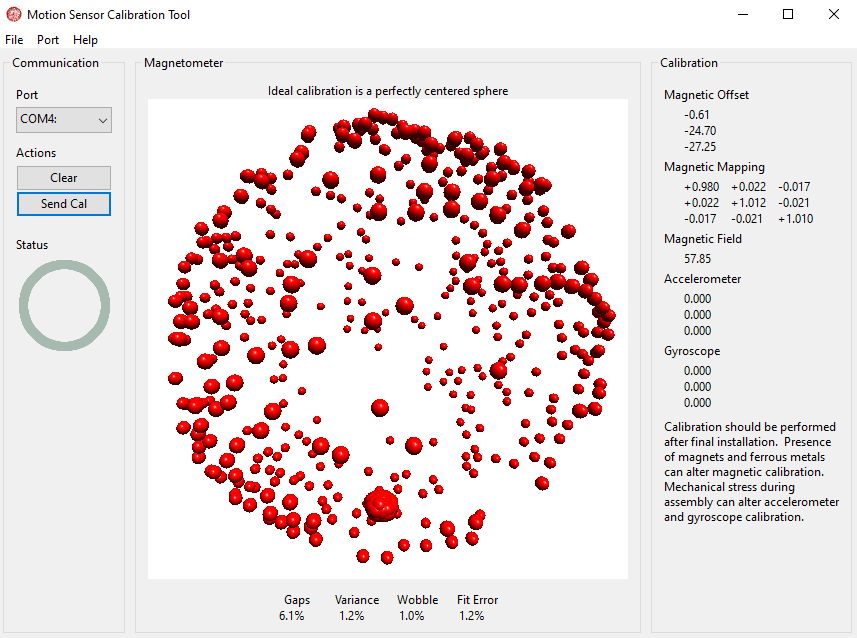
\includegraphics[width=0.9\textwidth]{images/6_design_final/sensor_calibration.png}
	\caption{Motion Sensor Calibration Tool by \textit{PJRC}}
	\label{fig:sensor_calibration_tool}
\end{figure}

\newpage
\subsection{Human Machine Interface (HMI)}
The \acrfull{hmi} of the mainboard consists of 17 \acrshort{rgb} \acrshort{led}s, with one specifically dedicated as a Status \acrshort{led}.
To provide acoustic feedback, a buzzer is integrated into the design.
This buzzer is particularly useful for alerting users to specific events, such as an audio buffer overflow, by playing a distinctive beep sequence.
Table \ref{tab:system_status_led} provides an overview of the \acrshort{led} indication patterns for the various system states.
\begin{table}[h!]
	\centering
	\begin{tabular}{ l l l l l}
		\textbf{System Status} & \textbf{Blink Pattern} & \textbf{LED Color} & \textbf{Streaming State} & \textbf{GNSS Fix} \vspace{0.1cm} \\ \hline
		Running                & 1 Pulse/Second         & White              & No                       & No                               \\ \hline
		Running                & 2 Pulse/Second         & White              & Yes                      & No                               \\ \hline
		Running                & 1 Pulse/Second         & Green              & No                       & Yes                              \\ \hline
		Running                & 2 Pulse/Second         & Green              & Yes                      & Yes                              \\ \hline
		Warning                & 2\,Hz Blinking         & Yellow             & -                        & -                                \\ \hline
		Error                  & 2\,Hz Blinking         & Red                & -                        & -                                \\ \hline
	\end{tabular}
	\caption{System Status LED Indication}
	\label{tab:system_status_led}
\end{table}

\subsection{Graphical User Interface (GUI)}
The \acrshort{gui} provides a user-friendly interface for configuring the device and monitoring its status.
It is based on the acquisition system's \acrshort{gui} and makes again use of the \textit{lvgl} framework.

\subsection{GUI Pages}
In the following sections, the different \acrshort{gui} pages are explained in detail.
Navigating between the pages is done by clicking on the corresponding icon in the home menu.
To return to the home menu, the sub-page header bar with the arrow symbol can be pressed.
Figure \ref{fig:gui_pages_overview} shows an overview of all \acrshort{gui} pages and how navigation between them is done.
\begin{figure}[h!]
	\centering
	\vspace{-0.5cm}
	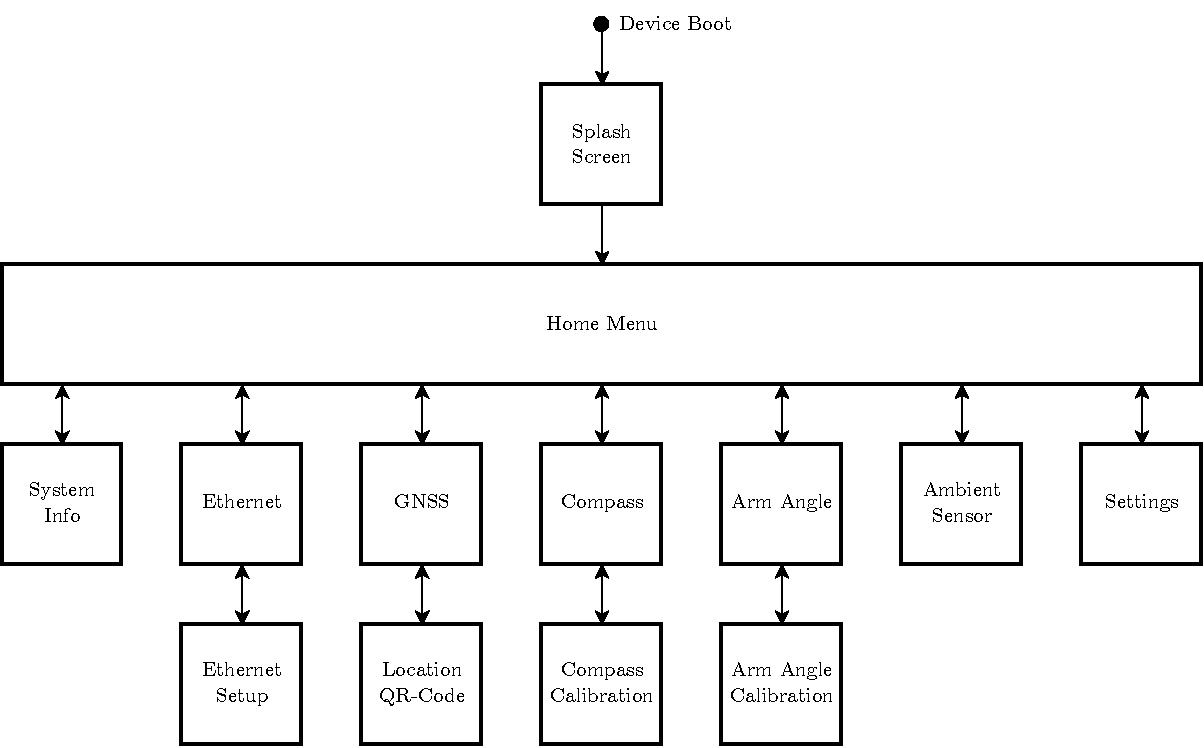
\includegraphics[width=0.86\textwidth]{images/6_design_final/final_design_gui_pages.pdf}
	\caption{GUI Pages Overview}
	\label{fig:gui_pages_overview}
\end{figure}
\newpage

\begin{minipage}{\linewidth}
	\begin{wrapfigure}{l}{4.5cm}
		\vspace{-0.6cm}
		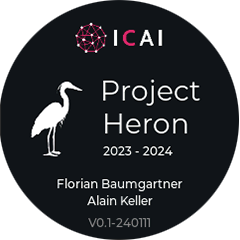
\includegraphics[width=4cm]{images/6_design_final/gui/00_splash_screen.png}
		\centering
		\caption{Splash Screen}
		\label{fig:final_design_gui_splash_screen}
	\end{wrapfigure}
	\subsubsection{Splash Screen}
	When the system is powered on, the splash screen is displayed for 5 seconds.
	On the bottom of the screen, the current firmware version and build date is displayed.
	After the system has booted, the home menu is displayed.
\end{minipage}
\vspace{2.0cm}		% One line corresponds to ca. 0.4cm

\begin{minipage}{\linewidth}
	\begin{wrapfigure}{l}{4.5cm}
		\vspace{-0.6cm}
		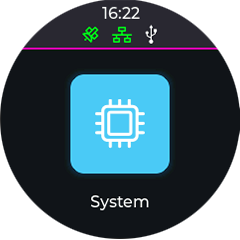
\includegraphics[width=4cm]{images/6_design_final/gui/01_main_menu.png}
		\centering
		\caption{Home Menu}
		\label{fig:final_design_gui_home_menu}
	\end{wrapfigure}
	\subsubsection{Home Menu}
	The home menu presents an intuitive way of navigating through the different submenus.
	On the top of the screen, the current time is displayed.
	A dedicated icon for the \acrshort{gnss}, ethernet and \acrshort{usb} interface is shown.
	Per default, the icons are grayed out.
	When the \acrshort{gnss} location is valid (fix), the icon turns green.
	When the device is connected to the network but is not yet streaming, the icon is filled white.
	As soon as the audio stream is active, the icon turns green.
	The \acrshort{usb} icon is filled white when a device is connected to the \acrshort{usb} port.
	As soon as the virtual COM port is opened, the icon turns green.
\end{minipage}
\vspace{0.1cm}

\begin{minipage}{\linewidth}
	\begin{wrapfigure}{l}{4.5cm}
		\vspace{-0.6cm}
		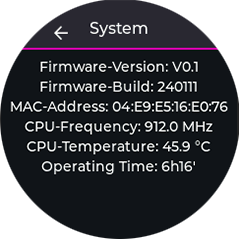
\includegraphics[width=4cm]{images/6_design_final/gui/03_system_info.png}
		\centering
		\caption{System Information}
		\label{fig:final_design_gui_system_info}
	\end{wrapfigure}
	\subsubsection{System Information}
	The system information page displays important device information such as the firmware version,
	firmware build date, etherent \acrshort{mac} address, \acrshort{cpu} frequency and temperature, as well as the operating time.
\end{minipage}
\vspace{2.1cm}

\begin{minipage}{\linewidth}
	\begin{wrapfigure}{l}{4.5cm}
		\vspace{-0.6cm}
		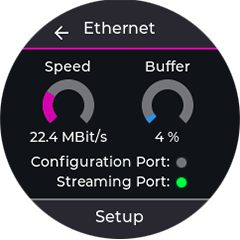
\includegraphics[width=4cm]{images/6_design_final/gui/04_ethernet.png}
		\centering
		\caption{Ethernet}
		\label{fig:final_design_gui_ethernet}
	\end{wrapfigure}
	\subsubsection{Ethernet}
	The ethernet page displays the current connection state of the streaming and configuration port.
	While a connection is established to either of the ports, the corresponding gray circle is filled green.
	Two gauge bars display the current streaming speed and the fill level of the streaming buffer.
	In normal operation, the indicated streaming speed should be around 22\,Mbit/s and the buffer fill level near 0\,\%.
\end{minipage}
\newpage

\begin{minipage}{\linewidth}
	\begin{wrapfigure}{l}{4.5cm}
		\vspace{-0.6cm}
		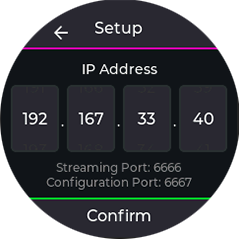
\includegraphics[width=4cm]{images/6_design_final/gui/05_ethernet_config.png}
		\centering
		\caption{Ethernet Setup}
		\label{fig:final_design_gui_ethernet_setup}
	\end{wrapfigure}
	\subsubsection{Ethernet Setup}
	The ethernet setup page allows for configuring the \acrshort{ip} address  of the device.
	Below the \acrshort{ip} address, the hard-coded streaming port (6666) and configuration port (6667) is displayed.
	When the \acrshort{ip} address is changed, the user can either confirm the change or discard it by returning to the previous page.
	When a new \acrshort{ip} address is confirmed, the device will instantly change its \acrshort{ip} address and restart the servers.
\end{minipage}
\vspace{0.2cm}

\begin{minipage}{\linewidth}
	\begin{wrapfigure}{l}{4.5cm}
		\vspace{-0.6cm}
		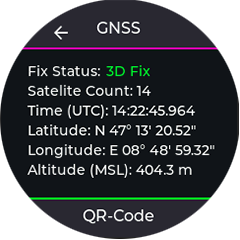
\includegraphics[width=4cm]{images/6_design_final/gui/06_gnss.png}
		\centering
		\caption{GNSS}
		\label{fig:final_design_gui_gnss}
	\end{wrapfigure}
	\subsubsection{GNSS}
	The \acrshort{gnss} page displays the current status of the \acrshort{gnss} module.
	When the Fix Status is valid (2D-Fix or 3D-Fix), the latitude, longitude and altitude is displayed.
	In addition, the QR-Code button gets enabled, which allows for displaying the current location in a QR-Code.
	The coordinates are displayed in degrees, minutes and seconds.
	The altitude is displayed in meters above sea level (MSL).
	When the time is fully resolved, it is displayed in the UTC+0 format.
	While the Fix Status is invalid, all fields are grayed out.
\end{minipage}
\vspace{0.0cm}

\begin{minipage}{\linewidth}
	\begin{wrapfigure}{l}{4.5cm}
		\vspace{-0.6cm}
		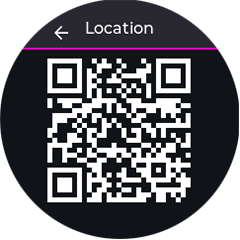
\includegraphics[width=4cm]{images/6_design_final/gui/07_gnss_location.png}
		\centering
		\caption{Location QR-Code}
		\label{fig:final_design_gui_gnss_location}
	\end{wrapfigure}
	\subsubsection{GNSS Location QR-Code}
	The \acrshort{gnss} location \acrshort{qrcode} page displays a \acrshort{qrcode} containing a google maps link to the current location.
	When the \acrshort{qrcode} is scanned with a smartphone, the web broweser will immediately redirect the user to the google maps app.
	The \acrshort{url} is formated as follows: \smallskip \newline
	\codeword{google.com/maps/place/<latitude>,<longitude>} \smallskip \newline
	For example, the \acrshort{url} directs to: \smallskip \newline
	\url{google.com/maps/place/47.222400,8.816460}
\end{minipage}
\vspace{0.0cm}

\begin{minipage}{\linewidth}
	\begin{wrapfigure}{l}{4.5cm}
		\vspace{-0.6cm}
		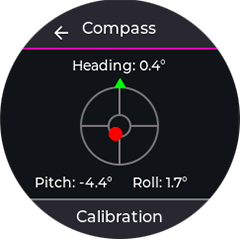
\includegraphics[width=4cm]{images/6_design_final/gui/08_compass.png}
		\centering
		\caption{Compass}
		\label{fig:final_design_gui_compass}
	\end{wrapfigure}
	\subsubsection{Compass}
	The compass page displays the current heading and leveling of the device.
	The heading is indicated by a purple arrow, pointing towards geographic north.
	When the needle points exactly towards the top of the screen it turns green, meaning the device is facing north.
	The circular graphic in the centre of the screen shows the current leveling of the device.
	When the device is perfectly leveled, the circle turns green.
	When the device is tilted, the circle turns red and the tilt angle is displayed in degrees (pitch and roll).
	To calibrate the built-in magnetometer, the user can press the calibrate button.
\end{minipage}
\vspace{-0.2cm}

\begin{minipage}{\linewidth}
	\begin{wrapfigure}{l}{4.5cm}
		\vspace{-0.6cm}
		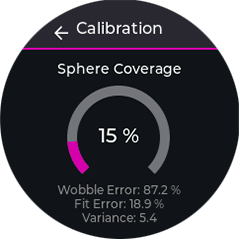
\includegraphics[width=4cm]{images/6_design_final/gui/09_compass_calibration.png}
		\centering
		\caption{Compass Calib.}
		\label{fig:final_design_gui_compass_calibration}
	\end{wrapfigure}
	\subsubsection{Compass Calibration}
	The compass calibration page displays the current status of the magnetometer calibration.
	By entering this page, the calibration process is starts immediately.
	To calibrate the magnetometer, the device has to be rotated around all three axes.
	This process takes around 30 seconds.
	As soon as the spere coverage indicator reaches 100\,\%, the calibration is finished, a success message is displayed and the buzzer plays a short melody.
	The calibration process can be aborted at any time by returning to the previous page (the calibration progress is not saved).
\end{minipage}
\vspace{-0.2cm}

\begin{minipage}{\linewidth}
	\begin{wrapfigure}{l}{4.5cm}
		\vspace{-0.6cm}
		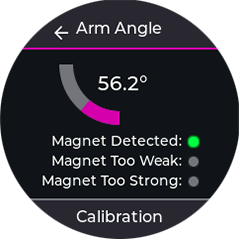
\includegraphics[width=4cm]{images/6_design_final/gui/10_angle_sensor.png}
		\centering
		\caption{Arm Angle}
		\label{fig:final_design_gui_arm_angle}
	\end{wrapfigure}
	\subsubsection{Arm Angle}
	The arm angle page displays the current angle of the microphone array arms in degree.
	When the arms are fully unfolded (horizontal) the angle is 0.0\,°.
	When the arms are fully folded towards the centre pole the angle is 90.0\,°.
	Below the angle indicator, the current status of the magnet detection is displayed.
	When the magnet is detected, the status indicator turns green.
	If the magnet is too weak or too strong, the corresponding status indicator turns yellow.
	Otherwise, the status indicators are grayed out.
\end{minipage}
\vspace{0.0cm}

\begin{minipage}{\linewidth}
	\begin{wrapfigure}{l}{4.5cm}
		\vspace{-0.6cm}
		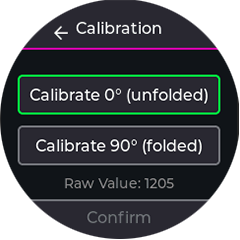
\includegraphics[width=4cm]{images/6_design_final/gui/11_angle_sensor_calibration.png}
		\centering
		\caption{Arm Angle Calib.}
		\label{fig:final_design_gui_arm_angle_calibration}
	\end{wrapfigure}
	\subsubsection{Arm Angle}
	The arm angle calibration page lets the user calibrate the angle sensor.
	To calibrate the angle sensor, the arms have to be fully unfolded (horizontal).
	Then the upper calibrate button \textit{Calibrate 0° (unfolded)} has to be pressed.
	Next, the arms have to be fully folded towards the centre pole.
	Then the lower calibrate button \textit{Calibrate 90° (folded)} has to be pressed.
	To confirm the calibration, the user has to press the \textit{Confirm} button.
\end{minipage}
\vspace{0.0cm}

\begin{minipage}{\linewidth}
	\begin{wrapfigure}{l}{4.5cm}
		\vspace{-0.6cm}
		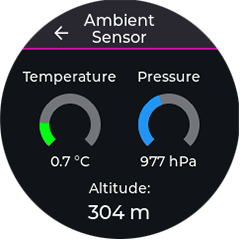
\includegraphics[width=4cm]{images/6_design_final/gui/12_ambient_sensor.png}
		\centering
		\caption{Ambient Sensor}
		\label{fig:final_design_gui_ambient_sensor}
	\end{wrapfigure}
	\subsubsection{Ambient Sensor}
	The ambient sensor page displays the current ambient temperature in degree Celsius and the ambient pressure in hectopascal.
	A gauge bar visualizes both values.
	Based on the current ambient pressure, the altitude above sea level is calculated and displayed in meters.
	Note that the altitude is only an approximation and can be inaccurate.
	It is strongly influenced by the current weather conditions.
\end{minipage}
\vspace{0.5cm}

\begin{minipage}{\linewidth}
	\begin{wrapfigure}{l}{4.5cm}
		\vspace{-0.6cm}
		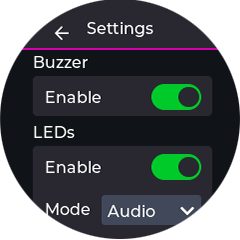
\includegraphics[width=4cm, trim={0 -1.0cm 0 0}]{images/6_design_final/gui/13_settings.png}
		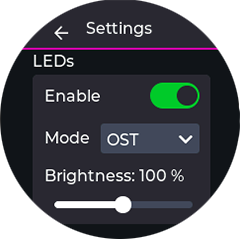
\includegraphics[width=4cm]{images/6_design_final/gui/14_settings.png}
		\centering
		\caption{Settings}
		\label{fig:final_design_gui_settings}
	\end{wrapfigure}
	\subsubsection{Settings}
	The settings page allows the user to configure the device.
	First, the buzzer can be enabled or disabled.
	Second, the \acrshort{led}s can be permanently enabled or disabled.
	The mode selection provides a selection of different animations for the \acrshort{led}s.
	Currently, there are two animation types implemented:
	\begin{itemize}
		\setlength{\itemindent}{5mm}
		\setlength{\leftmargin}{10mm}
		\item \textbf{Audio:} The \acrshort{led}s are controlled by the audio level of the microphone array.
		\item \textbf{OST:} The \acrshort{led}s show a fluent animation in the \acrshort{ost} color scheme.
	\end{itemize}
	Below the mode settings, the \acrshort{led} brightness can be adjusted.
	All settings are saved in the internal flash memory of the device and are restored after a reboot.
\end{minipage}
\newpage


\section{Software Design}
\label{chap:fin:sw}
The software is made to perform the tracking of the sound sources.
It runs on a external device, in this case a Dell Latitude 5310 Laptop
with Ubuntu installed.

\subsection{Audio Interface}
The Audio Interface provides the application with the audio data
from either the TCP stream or a pre recorded WAV FIle.
In both methods, the data is stored into an adapted ring buffer
until it is used by the main application.
\subsubsection{Ring Buffer}
A slightly modified ring buffer has been implemented to buffer the
audio data.
It is thread save since the storing and reading functions are called from
different threads.
The main difference to a conventional ring buffer is that the data is not
read from the tail but rather from the head.
This allows the application to always read the last $N$ samples while the data
in the buffer does not get split up.

Additionally the ringbuffer is able to write newly input data into a
WAV file.

\subsubsection{TCP Stream}
The TCP streamer allows to stream the audio directly via TCP form the microphone array.
The streaming runs via a socket to which the application connects to.
Using the control sequence the received data is preprocessed and then stored into
the buffer.

\subsubsection{WAV Stream}
The WAV stream is made with the PYAudio and the WAVE library from python.
With the WAVE library a .wav file is opened and then
played back with PYAudio.
Via a callback in the played audio is also stored into the ring buffer.
On windows and MacOs PYAudio could not stream a 32 channel WAV file.
Hence the application needs to be ran on Ubuntu.
Other Linux distributions may also work but were not tested during
this thesis.

\subsection{Communication}
To retrieve the sensor data from the microphone array
a communicator class was created.
It continuously reads the JSON containing various data
via a POST request from the microphone array.

\subsection{Sound Source Tracking}
The sound source tracking consists of three parts, the beamforming, peak detector and
Kalman Tracker.

\subsubsection{Beamforming}
First a data block is ran through the beamforming filterbank.
Contrary to prior beamforming grid, a pseudo uniformly sampled
semisphere is used to define the steering angles.
During testing, a samplenumber of 1700 points, which
gives an angle resolution of $\approx 2^\circ$, was used.
The number can be adjusted if higher resolution is necessary.
With these samples and the current array arm angle, the filterbank can be
calculated.
The beamforming used is the Delay and Sum beamforming,
which gives a power level for each steering direction.

\subsubsection{Peak Detection}
To detect where possible sound source are, a peak detector was implemented.
If only one source needs to be tracked, a simple argmax on the beamforming
response is sufficient.

For the case of multiple sources a more elaborate peakdetector is used.
To simplify the peakdetector, the beamformer response, which is defined on
a sphere is mapped onto a flat surface with
\begin{align}
	x & = \theta \cos\phi  \\
	y & = \theta \sin\phi.
	\label{eq:maping}
\end{align}
This mapping is later also used for the Kalmann tracker.
The mapped response is then converted to an image with linear interpolation.
This image allows the use of a 2d peak detector like the one described in
\cite{cvpeakdet}.
The basic function is to use grayscale dilation to find local maxima
and then filter out larger plateaus with a
median blur filter.
The resulting peaks can be further filtered by minimal height and
minimal ratio to the maximum value.
Other filters may be useful in the future, but were not implemented in this version.

\subsubsection{Kalman Tracker}
The found peaks are given to the Kalman Tracker.
With the Hungarian method the peaks are assigned to their corresponding
trackers.
If a existing tracker does not correspond to a peak, the Kalman
Filter can predict it's new position.
By default it makes ten such blind predictions until the track is discarded.

\subsection{GUI}
To visualize the beamforming responses and control the tracker a web based \acrshort{gui} with
Plotly and Dash was created.
Figure \ref{fin:fig:gui} shows a screenshot of the \acrshort{gui} while tracking is performed
on a pre recorder WAV file.
With the \acrshort{gui} and the current tracker settings the software runs on 5 \acrshort{fps}.
\begin{figure}
	\centering
	%    \includegraphics[width=0.25\textwidth]{mesh}
	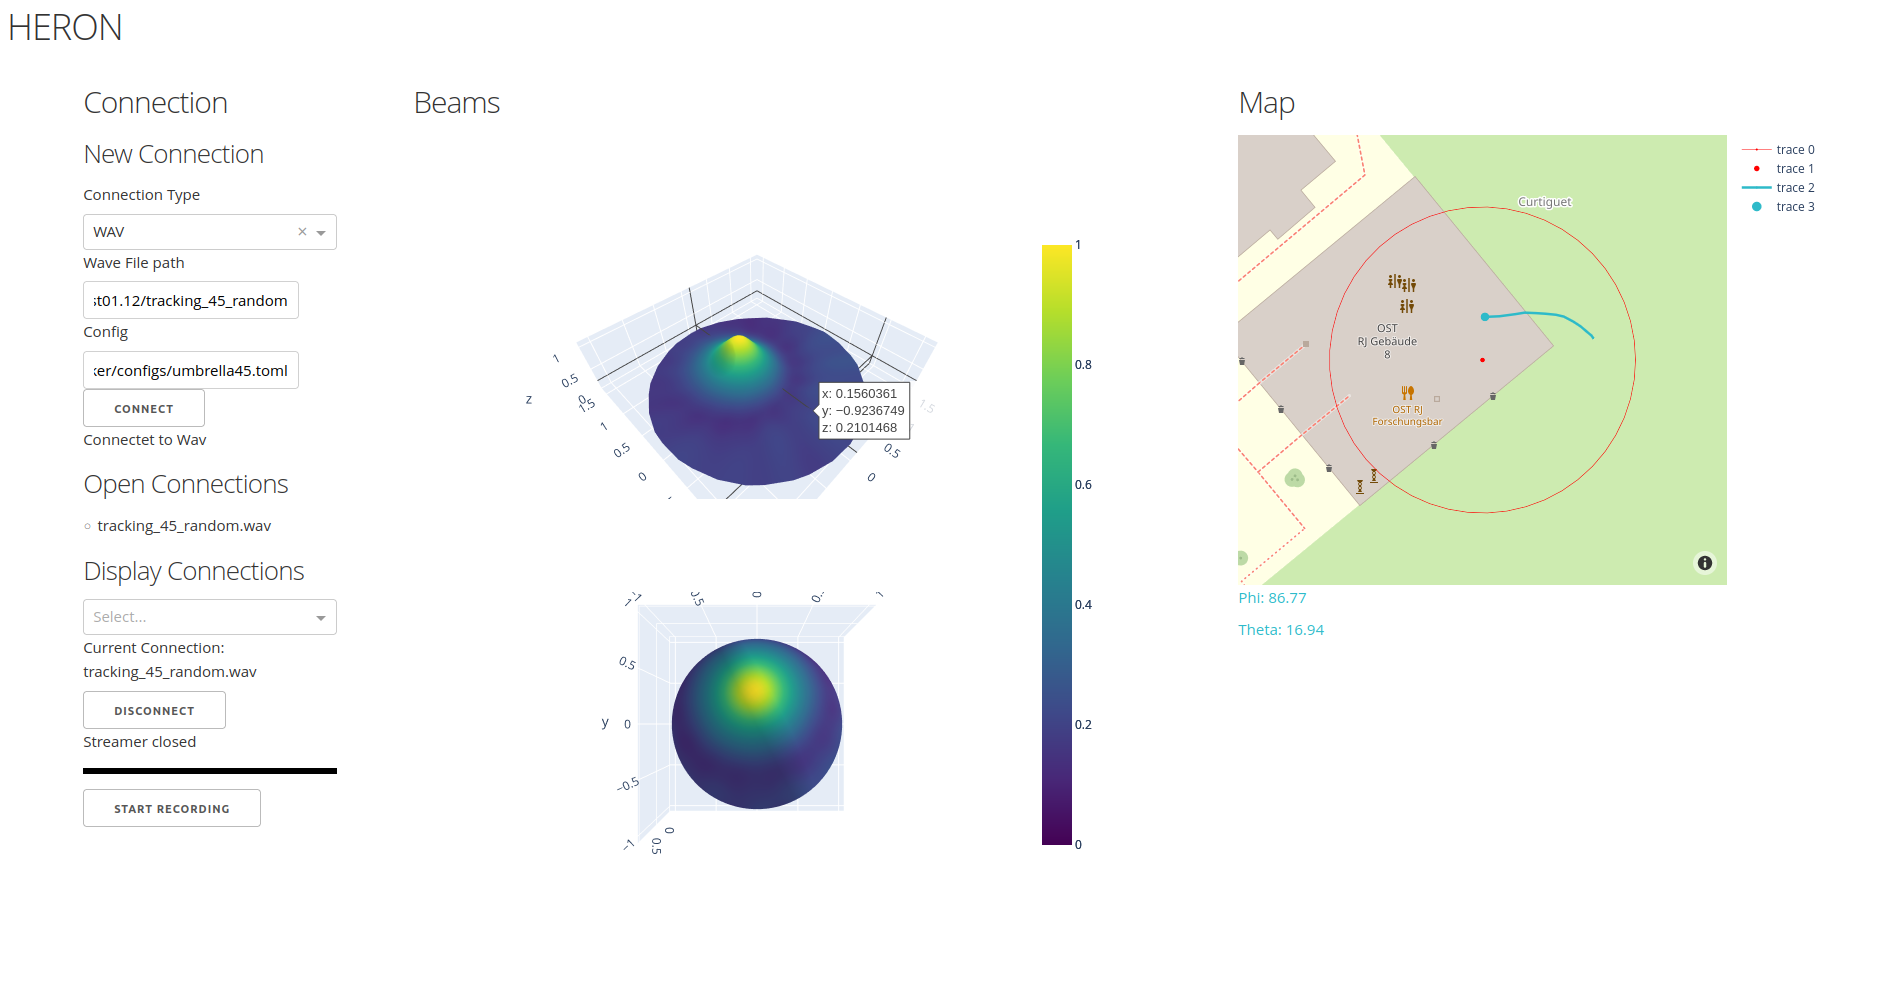
\includegraphics[width=14.2cm]{images/6_design_final/gui.png}
	\caption{Screenshot of the GUI.}
	\label{fin:fig:gui}
\end{figure}

\subsubsection{Connections}
On the left side the user can manage the connections to the audio streamer.
New connections to a Wav streamer can be established by providing a audio file
and an array configuration. To open a TCP connection, the IP address and port
of the array is needed.
Connections can also be closed with the \textit{close connection} button.

Open connections are listed below and via a dropdown list,
the displayed connection can be selected.

The streamed audio data can be recorded to a WAV file with the \textit{Start Recording}
button.

\subsubsection{Beamforming}
The beamforming response is shown in two different ways.
The top plot shows the mapped beamforming response in a surface plot, where
the z-axis represents the beamformed power.
To increase readability the power is normalized between zero and one.
The bottom plot displays the sampled semisphere where the color
represents the beamformed power.

\subsubsection{Map}
The map shows the current position of the array.
If no GPS data is available the default position is by the
building 8 at OST in Rapperswil.
The tracks are also displayed on the map.
Since with one array the exact position of the sound source
can not be determined, the directions are mapped onto the map with
\ref{eq:maping}.
To make the circle bigger, $\theta$ is multiplied by 30 before mapping it.
The red circle indicates a $\theta = 90^\circ$.
By using the compass data, the alignment of the array does not matter
for the tracks to be displayed in the right compass direction.

If the external does not have an internet connection to display the map,
the application can be run in an offline mode.